% Compile from this directory: make slides
% Speaker edition: make notes
\documentclass[aspectratio=169,11pt]{beamer}
\usepackage[T1]{fontenc}
\usepackage{lmodern,amsmath,amssymb,bm,booktabs,mathtools,array}
\usepackage{tikz,pgfplots}
% The build tool writes this auxiliary file from the verified reference snapshot.
\usepackage{xr}
\externaldocument[thesis-]{thesis-labels}
\newcommand{\dref}[2]{#1~\ref*{thesis-#2}}
\newcommand{\drefpage}[1]{p.~\pageref*{thesis-#1}}
\ifdefined\DefenseNotes\else
  \ifdefined\DefensePresenter\usepackage{multimedia}\else\usepackage{animate}\fi
\fi
\usetikzlibrary{arrows.meta,positioning,calc}
\pgfplotsset{compat=1.18}
\graphicspath{{./}}
\pdfstringdefDisableCommands{\def\translate#1{#1}}
\definecolor{ink}{HTML}{172F46}
\definecolor{teal}{HTML}{007F83}
\definecolor{amber}{HTML}{BD672A}
\definecolor{soft}{HTML}{EDF5F5}
\definecolor{muted}{HTML}{506576}
\setbeamercolor{normal text}{fg=ink,bg=white}
\setbeamercolor{structure}{fg=teal}
\setbeamercolor{frametitle}{fg=ink}
\setbeamercolor{title}{fg=ink}
\setbeamercolor{block title}{fg=white,bg=teal}
\setbeamercolor{block body}{fg=ink,bg=soft}
\setbeamercolor{alerted text}{fg=amber}
\setbeamerfont{title}{size=\LARGE,series=\bfseries}
\setbeamerfont{frametitle}{size=\Large,series=\bfseries}
\setbeamertemplate{navigation symbols}{}
\setbeamertemplate{blocks}[rounded][shadow=false]
\setbeamersize{text margin left=8mm,text margin right=8mm}
\setbeamertemplate{frametitle}{\vspace{2mm}\insertframetitle\par\vspace{1mm}\textcolor{teal}{\rule{\textwidth}{0.6pt}}}
\newif\ifbackup
\backupfalse
\newcommand{\routecrumb}[2]{\ifnum\value{section}=#1\textcolor{teal}{\textbf{#2}}\else\textcolor{muted}{#2}\fi}
\newcommand{\routeseparator}{\;\textcolor{muted}{$\rightarrow$}\;}
\setbeamertemplate{footline}{\hspace{8mm}\scriptsize\ifbackup\textcolor{muted}{Discussion}\hfill\textcolor{muted}{\insertframenumber}\else\routecrumb{1}{Sensor and data}\routeseparator\routecrumb{2}{Reconstruction}\routeseparator\routecrumb{3}{Optical flow}\routeseparator\routecrumb{4}{Stereo depth}\routeseparator\routecrumb{5}{Conclusions}\hfill\textcolor{muted}{\insertframenumber\,/\,\MainFrames}\fi\hspace{8mm}\vspace{3mm}}
\newcommand{\MainFrames}{36}
\newcommand{\R}{\mathbb R}
\newcommand{\norm}[1]{\left\lVert#1\right\rVert}
\newcommand{\A}{\mathbf A}
\newcommand{\B}{\mathbf B}
\newcommand{\K}{\mathbf K}
\newcommand{\M}{\mathbf M}
\newcommand{\W}{\mathbf W}
\newcommand{\Lam}{\bm\Lambda}
\newcommand{\vct}{\mathbf v}
\newcommand{\fL}{\mathbf f_L}
\newcommand{\fR}{\mathbf f_R}
\newcommand{\yL}{\mathbf y_L}
\newcommand{\yR}{\mathbf y_R}
\newcommand{\takeaway}[1]{\vspace{1.5mm}\begin{beamercolorbox}[sep=1.6mm,wd=\textwidth]{block body}\small\textbf{Takeaway.} #1\end{beamercolorbox}}
\newcommand{\src}[1]{\vfill{\fontsize{6.5}{8}\selectfont\color{muted}Dissertation: #1\par}}
\newcommand{\panel}[3]{\begin{minipage}{#1\textwidth}\centering\includegraphics[width=\linewidth,height=3.1cm,keepaspectratio]{#2}\par\vspace{1mm}{\small #3}\end{minipage}}
% Presenter commentary is embedded beside each frame and hidden in the audience edition.
\newcommand{\talknote}[3]{\note{\raggedright\textbf{Slide \insertframenumber. Purpose / pace:} #1\par\medskip\textbf{Talking points:} #2\par\medskip\textbf{Explanation / transition:} #3\par}}
\ifdefined\DefenseNotes
  \setbeameroption{show only notes}
  \setbeamertemplate{note page}[compressed]
\else
  \setbeameroption{hide notes}
\fi
\title{Variational and Optimization-based Approaches\\for Event-Based Vision Applications}
\subtitle{From unobserved modes to well-posed estimators}
\author{Daniel Blauvelt}
\institute{Department of Mathematics\quad\textbullet\quad George Mason University\\Dissertation Director: Harbir Antil}
\date{Dissertation Defense\quad\textbullet\quad Fall 2026}
\hypersetup{pdftitle={Daniel Blauvelt — Dissertation Defense},pdfauthor={Daniel Blauvelt},colorlinks=true,linkcolor=teal}
\begin{document}
% Every frame has presenter notes. Source labels refer to the dissertation,
% not to labels in this standalone presentation. A = unscaled first difference;
% B = flow data coefficient (renamed from A_data to prevent a notation collision).

\section{The inverse problems}
\begin{frame}[plain]
\titlepage
\talknote{Opening; about 30 seconds.}{The motivating question is how to estimate images, motion, and depth when the sensor reports changes rather than conventional image frames. The mathematical thread is the interaction of observation null spaces, regularization, and identifiability.}{The talk first introduces the sensor without assuming a computer-vision background, then develops the three inverse problems. The defense date is intentionally not specified beyond the semester.}
\end{frame}

\begin{frame}{Scenes recovered from brightness changes}
\centering
\begin{columns}[T]
\column{.32\textwidth}\centering
\vspace{1mm}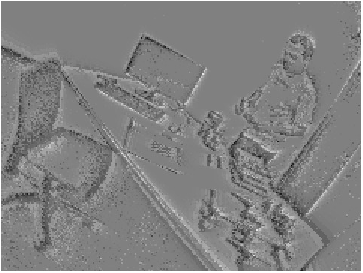
\includegraphics[width=\linewidth,height=3.6cm,keepaspectratio]{figures/office/office_ex_11.pdf}\par\vspace{.6mm}
% source: Ch. 2 subsubsec:datasets and subsec:validation_office; approx. 2.5M events.
{\footnotesize\textbf{Office}, handheld; $\approx2.5$M events}
\column{.32\textwidth}\centering
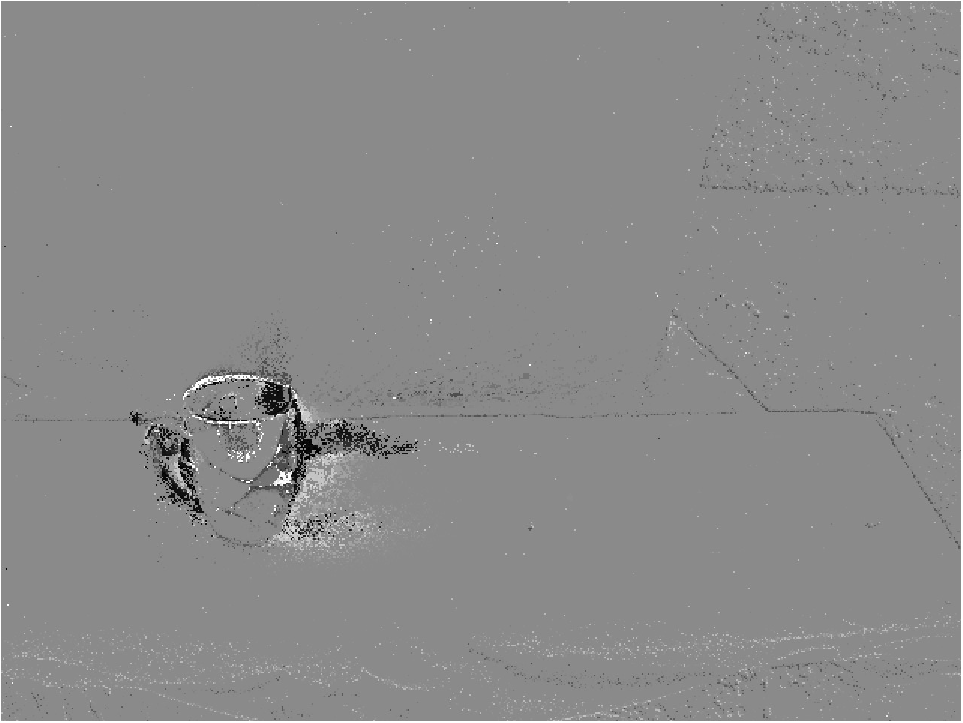
\includegraphics[width=\linewidth,height=1.85cm,keepaspectratio]{figures/cup/cup_ex_5.pdf}\par\vspace{.6mm}
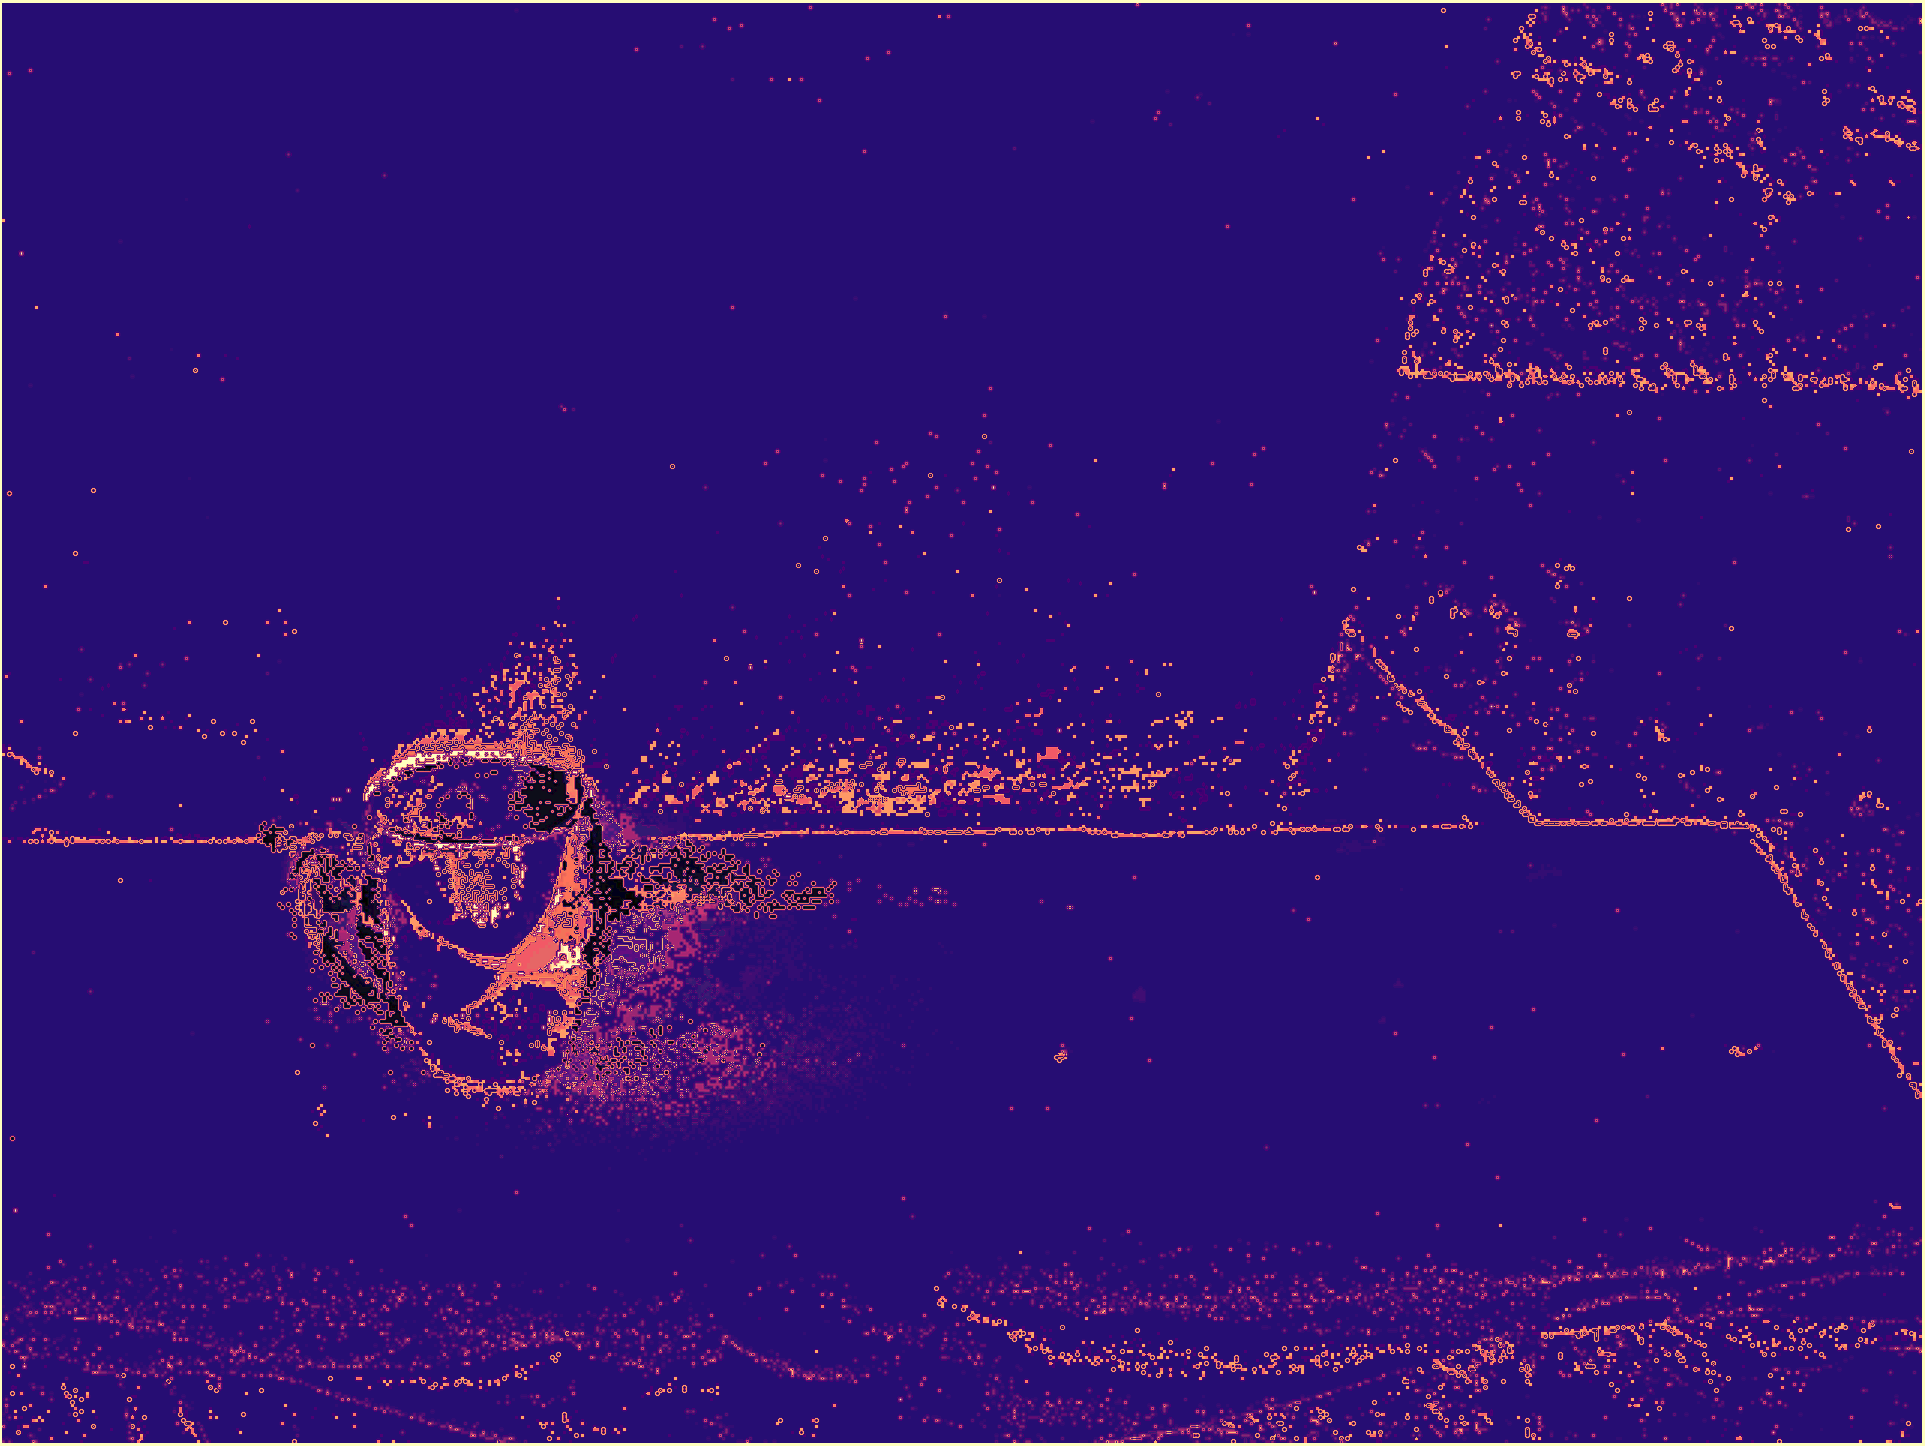
\includegraphics[width=\linewidth,height=1.85cm,keepaspectratio]{figures/cup/cm_cup/cup_5_0.0510_colormapped.png}\par
% source: Ch. 2 subsubsec:datasets and f:cup; approx. 350,000 events.
{\footnotesize\textbf{Bullet hits a cup}; $\approx350$K events}
\column{.32\textwidth}\centering
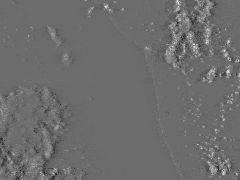
\includegraphics[width=\linewidth,height=1.85cm,keepaspectratio]{figures/ISS/110_0993g_reflected.png}\par\vspace{.6mm}
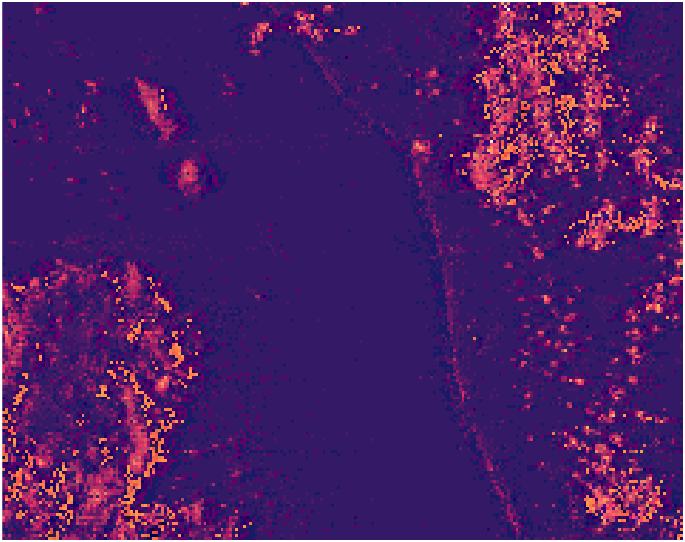
\includegraphics[width=\linewidth,height=1.85cm,keepaspectratio]{figures/ISS/110_0993_reflected.png}\par
% source: Ch. 2 subsubsec:datasets and f:iss; approx. 2 million events.
{\footnotesize\textbf{ISS} (Falcon Neuro); $\approx2$M events}
\end{columns}
{\scriptsize\color{muted}Cup and ISS: grayscale (top) and false color (bottom) of the same reconstructed frame.\par}
\vspace{1mm}\raggedright\small
% source: Gallego et al., "Event-based Vision: A Survey," IEEE TPAMI 44(1), 2022, abstract: microsecond temporal resolution, low power consumption.
Each pixel reports when its brightness changes, with microsecond timing and low power~\cite{gallego2022event}.\par\smallskip
This dissertation recovers images, motion, and depth from these changes, with guarantees on the estimates and computation simple enough for on-board use.
% source detail: Ch. 2, subsec:validation, f:office, f:cup, f:iss; datasets in subsubsec:datasets.
\src{\dref{Figure}{f:office}, \dref{Figure}{f:cup}, and \dref{Figure}{f:iss}; \dref{Section}{subsec:validation}. Data: office~\cite{gallego2017accurate}, cup~\cite{rebecq2021highspeed}, Falcon Neuro~\cite{mcharg2022falcon}.}
\talknote{Motivation; about 2 minutes. Show the results before any mathematics.}{Office: a handheld camera in an office; the desk objects and the person are recognizable. Cup: a bullet strikes a ceramic cup from the left; the event stream resolves the fracture and spray, which a standard-rate frame camera would blur. ISS: the Falcon Neuro event cameras on the International Space Station viewing the eastern coastline of Honduras; land--water boundaries and clouds are visible although the scene changes slowly and the events are sparse. All three come from events alone, with one per-pixel solve and no intensity frames.}{Why it matters: fast scenes, wide brightness ranges, and platforms with tight power budgets such as drones and spacecraft. On those platforms the estimator must also be cheap and predictable, which the reconstruction chapter quantifies. Grayscale and false color are display choices, not calibrated brightness. Transition: what the sensor reports, and why that makes these problems mathematically interesting.}
\end{frame}

\begin{frame}{Why an event camera? Each pixel reports its own changes}
\begin{columns}[T]
\column{.48\textwidth}
\centering\textbf{Conventional camera}\par\smallskip
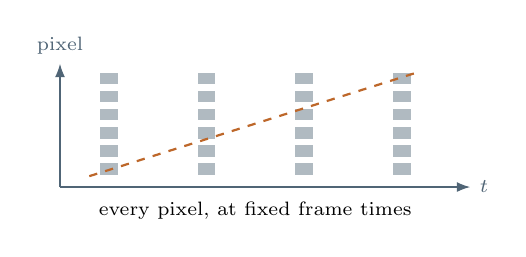
\begin{tikzpicture}[x=.62cm,y=.23cm,>=Latex]
\draw[->,muted] (0,0)--(8.4,0) node[right,font=\scriptsize] {$t$};
\draw[->,muted] (0,0)--(0,6.8) node[above,font=\scriptsize] {pixel};
\foreach \t in {1,3,5,7}{\foreach \r in {1,...,6}{\fill[muted!45] (\t-.18,\r-.32) rectangle (\t+.18,\r+.32);}}
\draw[amber,dashed,thick] (.6,.6)--(7.4,6.4);
\node[font=\scriptsize,align=center] at (4,-1.3) {every pixel, at fixed frame times};
\end{tikzpicture}
\column{.48\textwidth}
\centering\textbf{Event camera}\par\smallskip
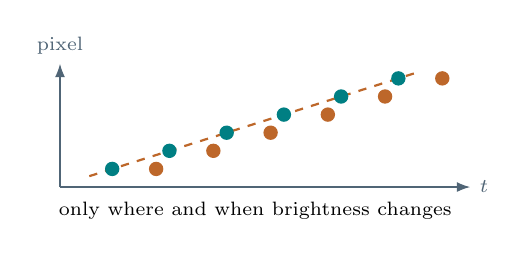
\begin{tikzpicture}[x=.62cm,y=.23cm,>=Latex]
\draw[->,muted] (0,0)--(8.4,0) node[right,font=\scriptsize] {$t$};
\draw[->,muted] (0,0)--(0,6.8) node[above,font=\scriptsize] {pixel};
\draw[amber,dashed,thick] (.6,.6)--(7.4,6.4);
\foreach \r in {1,...,6}{\fill[teal] ({.6+(\r-.6)*6.8/5.8},\r) circle (2.6pt);\fill[amber] ({.6+(\r-.6)*6.8/5.8+.9},\r) circle (2.6pt);}
\node[font=\scriptsize,align=center] at (4,-1.3) {only where and when brightness changes};
\end{tikzpicture}
\end{columns}
\vspace{-1mm}
{\footnotesize Dashed line: the leading edge of a moving bright bar. Teal: brightening ($+$); amber: darkening ($-$).}
\begin{itemize}\footnotesize
% source: Gallego et al., "Event-based Vision: A Survey," IEEE TPAMI 44(1), 2022, abstract (gmuETD.bib gallego2022event).
\item Microsecond timestamps, about $140$\,dB dynamic range versus $60$\,dB, low power, little motion blur~\cite{gallego2022event}.
\end{itemize}
% source detail: Ch. 1; Ch. 2, Neuromorphic Cameras overview. Diagram is schematic.
\src{\dref{Chapter}{ch:monocular_reconstruction}, neuromorphic camera overview; Gallego et al.~\cite{gallego2022event}. Diagram is schematic.}
\talknote{Accessibility primer; about two minutes. Assume no event-camera background.}{Point to the left panel: a conventional camera samples every pixel at the same frame times, whether or not anything changes, and averages over its exposure. Point to the right panel: the same moving bright bar produces a brightening event when its leading edge reaches a pixel and a darkening event when its trailing edge leaves. This is why event displays often look like moving outlines: a boundary passing across a pixel changes its brightness, while a uniform region undergoing the same translation produces little activity. The sensor responds to temporal brightness change; illumination changes can also trigger events. The survey figures quoted on the slide are the standard sensor-class numbers from Gallego et al.\ (TPAMI 2022), not measurements made in this dissertation.}{Give the committee the one idea the whole talk uses: events record when the log-brightness at a pixel changed by a fixed amount, so the data determine changes and leave the starting brightness free. Then turn to the next slide for the exact threshold rule. If asked about hardware: the dissertation's MVSEC, office, and cup data come from DAVIS346 sensors, and the orbital data from the Falcon Neuro instrument on the ISS.}
\end{frame}

\begin{frame}{An event camera: each pixel reports threshold crossings}
\begin{columns}[c]
\column{.57\textwidth}
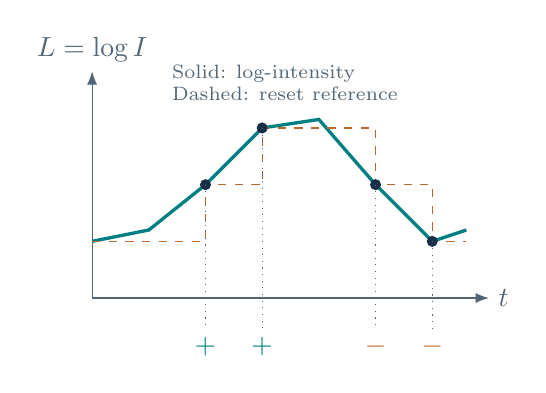
\begin{tikzpicture}[x=.72cm,y=.72cm,>=Latex]
\draw[->,muted] (0,0)--(7,0) node[right] {$t$};
\draw[->,muted] (0,0)--(0,4) node[above] {$L=\log I$};
\draw[teal,very thick] (0,1)--(1,1.2)--(2,2)--(3,3)--(4,3.15)--(5,2)--(6,1)--(6.6,1.2);
\draw[amber,dashed] (0,1)--(2,1)--(2,2)--(3,2)--(3,3)--(5,3)--(5,2)--(6,2)--(6,1)--(6.6,1);
\foreach \x/\y in {2/2,3/3,5/2,6/1}{\fill[ink] (\x,\y) circle (2pt);\draw[muted,dotted] (\x,\y)--(\x,-.55);}
\node[teal] at (2,-.85) {$+$};\node[teal] at (3,-.85) {$+$};
\node[amber] at (5,-.85) {$-$};\node[amber] at (6,-.85) {$-$};
\node[muted,align=left,font=\scriptsize] at (3.4,3.8) {Solid: log-intensity\\ Dashed: reset reference};
\end{tikzpicture}
\column{.40\textwidth}
An event is a tuple
\[e_k=(\mathbf x_k,s_k,p_k),\qquad p_k=\pm1.\]
For the ideal threshold model,
\[L(\mathbf x_k,s_k)-L(\mathbf x_k,s_k^-)=p_k c_{\rm th}.\]
The preceding reset $s_k^-$ is \textbf{local to that pixel}.
\end{columns}
% source detail: Ch. 2, eq:polarity; Ch. 3, eq:event\_integral. Diagram is schematic.
\src{\dref{Eq.}{eq:polarity}; \dref{Eq.}{eq:event_integral}; ideal threshold model~\cite{lichtsteiner2008128}. Diagram is schematic.}
\talknote{Sensor primer; 90 seconds.}{Follow the solid curve. A positive event is emitted after an upward change of one threshold from the most recent reset; a negative event follows a downward change. Different pixels have independent reset times, so the observation times are asynchronous. Neuromorphic here refers to the change-triggered sensing architecture; these estimators do not require a neural network.}{The equality is an ideal noiseless threshold model. Real threshold uncertainty, missed events, refractory effects, and overshoot create discrepancies. The diagram is conceptual, with arbitrary axes and no claim about measured latency. A stationary bright pixel can produce no events: zero activity is not zero intensity.}
\end{frame}

\begin{frame}{From events to images, motion, and depth}
\begin{columns}[T]
\column{.32\textwidth}
\centering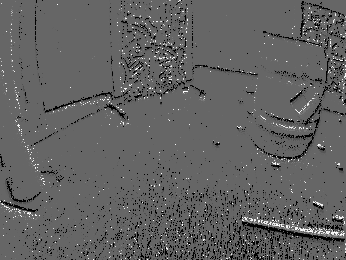
\includegraphics[width=\linewidth,height=2.1cm,keepaspectratio]{figures/indoor_flying2_t47p6/bspline_reconstruction.png}\par\vspace{1mm}
{\small\textbf{Image reconstruction}}\par
{\footnotesize Ch.\ 2}\par
{\scriptsize Grayscale: reconstructed value.}
\column{.32\textwidth}
\centering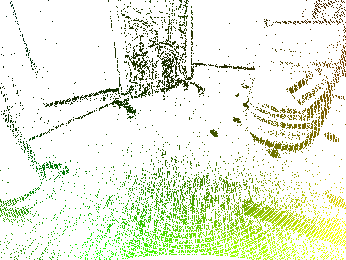
\includegraphics[width=\linewidth,height=2.1cm,keepaspectratio]{figures/indoor_flying2_t47p6/cmax_flow_event_pixels.png}\par\vspace{1mm}
{\small\textbf{Optical-flow estimate}}\par
{\footnotesize Ch.\ 3; event-active pixels}\par
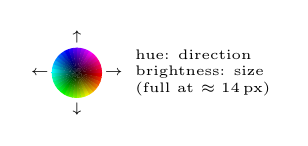
\begin{tikzpicture}[baseline=(wheel.center)]
\node[inner sep=0pt] (wheel) at (0,0) {\phantom{\rule{.7cm}{.7cm}}};
\foreach \a in {0,10,...,350}{%
  \pgfmathsetmacro{\hue}{\a/360}\definecolor{wheelhue}{hsb}{\hue,1,1}%
  \begin{scope}\clip (0,0)--(-\a:.32)--(-\a-11:.32)--cycle;
  \shade[inner color=black,outer color=wheelhue] (0,0) circle (.32);\end{scope}}
\node[font=\tiny,inner sep=1pt] at (0:.47) {$\rightarrow$};\node[font=\tiny,inner sep=1pt] at (-90:.46) {$\downarrow$};
\node[font=\tiny,inner sep=1pt] at (180:.47) {$\leftarrow$};\node[font=\tiny,inner sep=1pt] at (90:.46) {$\uparrow$};
\node[font=\tiny,align=left,anchor=west] at (.62,0) {hue: direction\\brightness: size\\(full at $\approx14$\,px)};
\end{tikzpicture}
\column{.32\textwidth}
\centering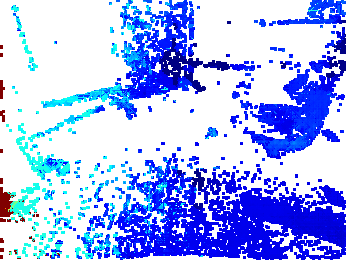
\includegraphics[width=\linewidth,height=2.1cm,keepaspectratio]{figures/indoor_flying2_t47p6/wls_depth.png}\par\vspace{1mm}
{\small\textbf{Stereo-depth estimate}}\par
{\footnotesize Ch.\ 4}\par
% source: figures/indoor_flying2_t47p6/metadata.json, wls_display.
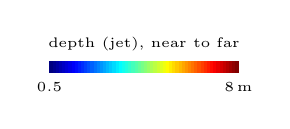
\begin{tikzpicture}
\foreach \i in {0,...,59}{\pgfmathsetmacro{\t}{\i/59}%
  \pgfmathsetmacro{\jr}{min(max(1.5-abs(4*\t-3),0),1)}\pgfmathsetmacro{\jg}{min(max(1.5-abs(4*\t-2),0),1)}\pgfmathsetmacro{\jb}{min(max(1.5-abs(4*\t-1),0),1)}%
  \definecolor{jetstep}{rgb}{\jr,\jg,\jb}\fill[jetstep] ({.04*\i},0) rectangle ({.04*\i+.05},.16);}
\node[font=\tiny,anchor=north] at (0,0) {$0.5$};\node[font=\tiny,anchor=north] at (2.4,0) {$8$\,m};
\node[font=\tiny,anchor=south] at (1.2,.16) {depth (jet), near to far};
\end{tikzpicture}
\end{columns}
\vspace{1mm}
% source: figures/indoor_flying2_t47p6/metadata.json, reconstruction and flow timestamps and WLS center.
{\footnotesize MVSEC~\cite{MVSEC2018} indoor\_flying2, drone-mounted event cameras, near $47.6$\,s; stereo depth uses both.}
% source detail: Saved HPC estimates; provenance, hashes, timestamps, display scales, and masks in figures/indoor_flying2_t47p6/metadata.json.
\src{Methods: \dref{Chapter}{ch:monocular_reconstruction}, \dref{Chapter}{ch:optical_flow}, and \dref{Chapter}{ch:stereo_depth_estimation}; MVSEC~\cite{MVSEC2018}.}
% source: figures/indoor_flying2_t47p6/metadata.json, timestamps, observation windows, display rules, and geometry.
\talknote{Accessibility primer; 90 seconds. Introduce the three estimated outputs.}{Left: temporal image reconstruction. Middle: optical-flow estimate, with color encoding direction and displacement magnitude at pixels that recorded events. Right: stereo depth. All three show the same indoor flying 2 scene. Present the panels as the three estimation targets. Explain the brightness baseline, motion along an edge, and stereo correspondence.}{If asked which methods: B-spline kernel with sigmoid weights; contrast maximization, whose nonconvex objective lies outside the quadratic family analyzed later (existence result in backup); weighted least squares. Reconstruction: 47.690 s. Flow: 47.592--47.719 s; color magnitude represents displacement over this window. White flow pixels have zero events: the mask shows event support, not confidence. WLS: center 47.598 s, 250 ms window. Different windows and stereo rectification permit scene-level comparison, with separate pixel geometries. Depth colors clip to 0.5--8 m; white masks nonfinite values and the maximum finite depth. Reconstruction grayscale uses a histogram/percentile scale. Exact timestamps, normalization, and provenance are in the adjacent metadata file.}
\end{frame}

\begin{frame}{Three estimators, each well posed}
\renewcommand{\arraystretch}{1.6}
\begin{tabular}{>{\raggedright\arraybackslash}p{3.7cm}>{\raggedright\arraybackslash}p{9.7cm}}
\textbf{Reconstruction} (Ch.~2) & One tridiagonal solve per pixel; unique and stable for every positive weight.\\
\textbf{Optical flow} (Ch.~3) & Three event representations, one quadratic theory; unique flow when edges span two directions.\\
\textbf{Stereo depth} (Ch.~4) & A unique inner solve at each candidate depth; competitive MVSEC accuracy with the most scored points.\\
\end{tabular}\par
\vspace{5mm}
{\small The common question: which quantities do the events determine, and which does the model supply?\par}
% source detail: Chs. 1 and 5; Ch. 5, tab:contribution\_matrix; Ch. 2 thm:uniqueness; Ch. 3 thm:unified\_wellposedness; Ch. 4 thm:weighted\_spd and App. tab:unified\_benchmark (2.66M scored points, the largest).
\src{\dref{Table}{tab:contribution_matrix}; \dref{Theorem}{thm:uniqueness}, \dref{Theorem}{thm:unified_wellposedness}, \dref{Theorem}{thm:weighted_spd}.}
\talknote{What the talk shows; about 90 seconds.}{Reconstruction gets most of the time: the model, its uniqueness and stability, and its cost. Optical flow follows with the main theorem. Stereo is a one-slide summary. Each row names a result, not a topic.}{The common question links the rows: the events determine some quantities, and the model supplies the rest. The footer tracks the position along this route. Start with the sensor's observation model, which is where the reconstruction begins.}
\end{frame}

\section{Temporal reconstruction}
\begin{frame}{Start with one pixel: integrated changes on a temporal chain}
\begin{columns}[T]
\column{.54\textwidth}
Choose a unit-mass temporal kernel $\phi_{s_k}$:
\[e(t)=\sum_{k\text{ at this pixel}}p_k\phi_{s_k}(t).\]
\[y_i=\int_{t_i}^{t_{i+1}}e(t)\,dt.\]
The reconstruction times $t_i$ are chosen by the algorithm.
\column{.43\textwidth}
\[\A=\begin{pmatrix}-1&1&&\\&-1&1&\\&&\ddots&\ddots\end{pmatrix}.\]
\[\A\mathbf f\approx\mathbf y.\]
\[\ker\A=\operatorname{span}\{\mathbf1\}.\]
Events determine increments, leaving a constant free.
\end{columns}
\vspace{1mm}
{\footnotesize\textbf{In scene terms:} each pixel's log-brightness history is rebuilt on its own from how much it rose or fell in each interval. The model chooses the reference level; a pixel without events stays at that level, whatever its brightness.\par}
% source detail: Ch. 2, eq:exy, eq:Exy, eq:tempdiffA, lem:nullspace.
\src{\dref{Eq.}{eq:Exy}, \dref{Eq.}{eq:tempdiffA}, and \dref{Lemma}{lem:nullspace}.}
\talknote{Temporal observation model; 75 seconds.}{Suppress the pixel index to keep the notation readable. Integrating a unit-mass kernel across a bin assigns all or part of each event to that bin. Delta binning has no spread; Gaussian, rectangular, and spline kernels distribute influence over time. The entries of A are unscaled increments, not derivatives divided by a time step.}{If Af=0, every consecutive pair of components is equal, hence f is constant. Conversely A1=0. Under ideal threshold calibration the observed increments approximate changes in L/c\_th, with kernel-boundary, overshoot, and between-event endpoint errors. No absolute frame is used to set the baseline. Scene terms: each pixel's brightness history is rebuilt on its own; a pixel without events stays at the reference level.}
\end{frame}

\begin{frame}{Temporal kernels: how far each event's influence spreads}
\begin{columns}[c]
\column{.50\textwidth}
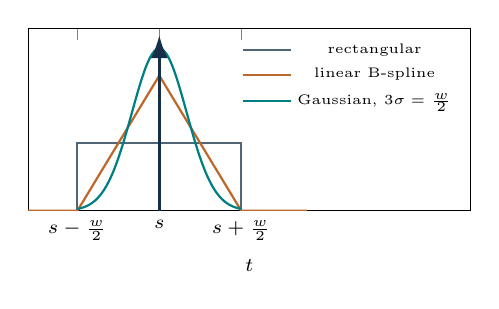
\begin{tikzpicture}
\begin{axis}[width=7.2cm,height=3.9cm,xmin=-.8,xmax=1.9,ymin=0,ymax=2.7,xtick={-.5,0,.5},xticklabels={$s-\frac w2$,$s$,$s+\frac w2$},ytick=\empty,xlabel={$t$},label style={font=\scriptsize},tick label style={font=\scriptsize},legend style={font=\tiny,at={(.99,.98)},anchor=north east,draw=none,fill=none}]
\addplot[muted,thick,const plot] coordinates {(-.8,0) (-.5,0) (-.5,1) (.5,1) (.5,0) (.9,0)};\addlegendentry{rectangular}
\addplot[amber,thick] coordinates {(-.8,0) (-.5,0) (0,2) (.5,0) (.9,0)};\addlegendentry{linear B-spline}
% source: analytic truncated Gaussian, sigma=w/6, Z=erf(3/sqrt 2)=0.9973 (Ch. 2 subsec:bumpsel).
\addplot[teal,thick,domain=-.5:.5,samples=80]{exp(-x^2/(2*(1/6)^2))/((1/6)*sqrt(2*pi)*0.9973)};\addlegendentry{Gaussian, $3\sigma=\frac w2$}
\draw[ink,very thick,-{Latex}] (axis cs:0,0)--(axis cs:0,2.6);
\end{axis}
\end{tikzpicture}
\par{\scriptsize Arrow: delta kernel (pure binning). Common support width $w$; schematic.}
\column{.47\textwidth}
\small Each kernel has unit mass, is a translate, and has compact support:
\[\int_{\R}\phi_s=1,\qquad \phi_s(t)=\phi_0(t-s).\]
Each event splits its sign $p_k$ across the bins it overlaps:
\[y_i=\sum_k p_k\int_{t_i}^{t_{i+1}}\phi_{s_k}(t)\,dt,\quad
\textstyle\sum_i y_i=\sum_k p_k\]
when every support lies inside $[t_0,t_N]$.
\end{columns}
% source detail: Ch. 2, subsec:bumpsel, prop:l1\_bump\_properties, prop:dist\_bump\_properties, tab:support\_widths.
\src{\dref{Proposition}{prop:l1_bump_properties}, \dref{Proposition}{prop:dist_bump_properties}; \dref{Table}{tab:support_widths}.}
\talknote{Kernel choice; 75 seconds.}{The four kernels are the ones evaluated in Chapter 2: delta (binning), truncated and renormalized Gaussian, B-spline, and rectangular. Unit mass means each event contributes exactly its sign in total; translation invariance means the bin integrals are a convolution; compact support means each event touches finitely many bins. The sum identity is exact: summing the bin integrals telescopes to the integral over the whole window, which is one when the event's full support lies in the window.}{The plotted widths are matched for display only; the evaluated parameters differ by kernel (Ch.\ 2 bump sweep). If asked which kernel is best: the indoor and outdoor rankings differ (discussion page on kernel performance), and the uniqueness theorem holds for every kernel because it depends only on $\A$ and positive weights. Transition: next, when these integrated observations approximate a physical brightness change.}
\end{frame}

\begin{frame}{From threshold crossings to an approximate observation}
\begin{columns}[c]
\column{.44\textwidth}
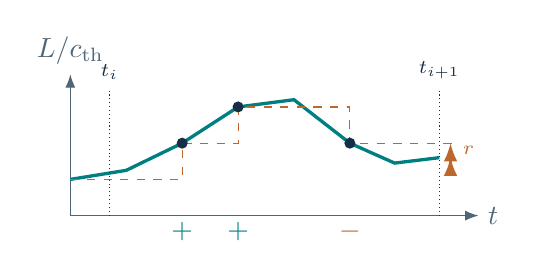
\begin{tikzpicture}[x=.71cm,y=.46cm,>=Latex]
\draw[->,muted] (0,0)--(7.3,0) node[right] {$t$};
\draw[->,muted] (0,0)--(0,3.9) node[above] {$L/c_{\rm th}$};
\draw[teal,very thick] (0,1)--(1,1.25)--(2,2)--(3,3)--(4,3.2)--(5,2)--(5.8,1.45)--(6.6,1.6);
\draw[amber,dashed] (0,1)--(2,1)--(2,2)--(3,2)--(3,3)--(5,3)--(5,2)--(6.9,2);
\foreach \x/\y in {2/2,3/3,5/2}{\fill[ink] (\x,\y) circle (2pt);}
\node[teal] at (2,-.45) {$+$};\node[teal] at (3,-.45) {$+$};\node[amber] at (5,-.45) {$-$};
\draw[ink,densely dotted] (.7,0)--(.7,3.5) node[above,font=\scriptsize] {$t_i$};
\draw[ink,densely dotted] (6.6,0)--(6.6,3.5) node[above,font=\scriptsize] {$t_{i+1}$};
\draw[amber,thick,<->] (6.8,1.6)--(6.8,2);
\node[amber,font=\scriptsize,anchor=west] at (6.85,1.8) {$r$};
\end{tikzpicture}\par
{\scriptsize Solid: $L/c_{\rm th}$. Dashed: reference at the last event.}
\column{.54\textwidth}
\small Ideal sensor: each event marks a log-brightness change of about one threshold $c_{\rm th}$.
\[y_i=\sum_k p_k\int_{t_i}^{t_{i+1}}\phi_{s_k}(t)\,dt\;\approx\;\frac{L(t_{i+1})-L(t_i)}{c_{\rm th}}.\]
Exactly, for any times $a<b$ at one pixel:
\end{columns}
\[\frac{L(b)-L(a)}{c_{\rm th}}=y(a,b)-\underbrace{B(a,b)}_{\text{\scriptsize kernel spill at bin edges}}+\underbrace{\frac1{c_{\rm th}}\sum_{a<s_\ell\le b}\varepsilon_\ell}_{\text{\scriptsize overshoot}}+\underbrace{r(b)-r(a)}_{\text{\scriptsize sub-threshold change}}.\]
% source detail: Ch. 2, subsubsec:physical_assumptions (P1)--(P4); subsubsec:physical, eq:qxylog, eq:vconnectq, arbitrary endpoint identity and regularized residual.
\src{Physical connection (\drefpage{subsubsec:physical}), \dref{Eq.}{eq:vconnectq}, arbitrary-endpoint identity; threshold model~\cite{lichtsteiner2008128}. Schematic diagram.}
\talknote{Sensor-to-observation model; about 90 seconds. Answers ``why is $\A\mathbf f\approx\mathbf y$ a model of an event camera?'' before it is asked.}{Under the ideal threshold rule each event marks a log-brightness change of one threshold, so the signed count between two times telescopes to the change in $L/c_{\rm th}$. The exact identity from Chapter 2 names the three discrepancies. $B$ is the kernel-boundary residual: kernel mass that spills across $t_i$ or $t_{i+1}$; it is zero for delta binning when no event lies on a boundary. $\varepsilon_\ell=\Delta_\ell-c_{\rm th}p_\ell$ is the overshoot at each recorded event. $r(t)$ is the unreported change since the most recent event; in the diagram it is the gap at $t_{i+1}$.}{Assumptions (P1)--(P4): unit-mass kernels, kernels localized relative to event spacing, $|\varepsilon_\ell|\ll c_{\rm th}$, and positive intensity. A missed or spurious event makes some $\varepsilon_\ell$ comparable to $c_{\rm th}$, which is outside (P3). The regularized solution adds a fourth discrepancy, the data residual: $f^*_k-f^*_i=y(t_i,t_k)+\sum_{\ell=i}^{k-1}\rho_{{\rm res},\ell}$, and larger weights enlarge it. Subthreshold signals can be invisible over a whole window: discussion page ``The physical event stream loses more than one baseline''. The measure-valued continuous-time limit is the discussion page on the jump primitive. Transition: the events fix changes, so a penalty must choose the level, which is the next theorem.}
\end{frame}

\begin{frame}{A unique, stable estimate for every positive weight}
\small
For fixed $\Lam=\operatorname{diag}(\lambda_i)$ with every $\lambda_i>0$,
\[\mathbf f^*=\arg\min_{\mathbf f\in\R^n}\ \tfrac12\norm{\A\mathbf f-\mathbf y}^2+\tfrac12\norm{\Lam\mathbf f}^2,\qquad
\K_{\rm time}=\A^\top\A+\Lam^\top\Lam\succeq\lambda_{\min}^2\mathbf I.\]
\begin{itemize}
\item \textbf{Unique:} the normal equations $\K_{\rm time}\mathbf f^*=\A^\top\mathbf y$ have exactly one solution.
% source: Ch. 2 prop:stability, ||A||_2 <= 2; one event changes y by at most 1 in norm.
\item \textbf{Stable:} $\norm{\delta\mathbf f^*}\le(2/\lambda_{\min}^2)\norm{\delta\mathbf y}$, so one spurious event moves a pixel's history by at most $2/\lambda_{\min}^2$.
% source: Direct consequence of Ch. 2 thm:uniqueness normal equations and A1=0; supplementary identity.
\item \textbf{Reference level:} $\mathbf1^\top\Lam^2\mathbf f^*=0$; quiet intervals carry the largest weights and set the level.
\end{itemize}
% source detail: Ch. 2, eq:in, thm:uniqueness, prop:stability.
\src{\dref{Eq.}{eq:in}, \dref{Theorem}{thm:uniqueness}, \dref{Proposition}{prop:stability}; Tikhonov regularization~\cite{tikhonov1977solutions}.}
\talknote{Theorem and stability; about 3 minutes.}{The objective balances fidelity to the observed changes against a weighted magnitude penalty. Its quadratic form is $\norm{\A\mathbf z}^2+\norm{\Lam\mathbf z}^2\ge\lambda_{\min}^2\norm{\mathbf z}^2$, so the normal matrix is positive definite and the minimizer is unique. Subtracting the normal equations for two data vectors gives $\delta\mathbf f^*=\K_{\rm time}^{-1}\A^\top\delta\mathbf y$ and, with $\norm{\A}_2\le2$, the stated bound.}{One spurious or missed event changes the data by at most one in norm, because each kernel splits a single unit of polarity across the bins. Premultiplying the normal equations by the constant vector gives the weighted zero-mean identity: the penalty selects the baseline and also changes the fitted increments. The derivation and the condition-number bound are in the backup "Why uniqueness and stability hold".}
\end{frame}

\begin{frame}{One tridiagonal solve per pixel}
\begin{columns}[T]
\column{.46\textwidth}
\small
$\A^\top\A$ has diagonal $(1,2,\dots,2,1)$ and off-diagonals $-1$, so
\[\K_{\rm time}=\A^\top\A+\Lam^\top\Lam\]
is tridiagonal and diagonally dominant.
\begin{itemize}\footnotesize\setlength{\itemsep}{2pt}
\item Thomas algorithm: $O(N)$ operations per pixel, no pivoting.
\item Pixels are independent; a pixel without events returns $\mathbf f=0$.
\item The newest frame comes from the forward sweep alone: constant work per pixel for each new interval.
\end{itemize}
\column{.51\textwidth}
\footnotesize\textbf{Measured on a laptop CPU}\par
{\scriptsize processing time $\div$ recording time; 100\,ms windows, $N=50$\par}\smallskip
% source: monocular_reconstruction/python/edge/README.md, laptop timings table (bench JSON in python/edge/results/: davis_pendulum T100ms N50, evk4_office T100ms N50; float32, active-pixel solve for DAVIS).
\begin{tabular}{lrrrr}\toprule Sensor & Pixels & Events/s & 1 core & 8 cores\\\midrule
DAVIS346 & 90k & 0.25\,M & 0.03 & 0.01\\
EVK4 & 922k & 13\,M & 2.5 & 0.67\\\bottomrule
\end{tabular}\par\medskip
% source: monocular_reconstruction/python/edge/README.md, Validation: cup, 500k events, 150 latent times; MATLAB lat_image_af_with_lambda.m 39.6 s, tridiagonal 0.22 s, max relative difference 6.6e-16.
Cup recording, 500k events, 150 frames: MATLAB reference 39.6\,s $\to$ 0.22\,s, same output to $10^{-15}$.
\end{columns}
% source detail: Ch. 2 eq:tempdiffA and thm:uniqueness (structure); monocular_reconstruction/python/edge (implementation, validation, timings).
\src{\dref{Eq.}{eq:tempdiffA}, \dref{Theorem}{thm:uniqueness}; Thomas algorithm~\cite{golub2013matrix}; timings: edge implementation, October 2026.}
\talknote{Cost; about 3 minutes. This answers the pre-defense question about edge hardware.}{The first-difference matrix makes $\A^\top\A$ the path-graph Laplacian; adding a positive diagonal keeps it tridiagonal and makes it diagonally dominant, so Gaussian elimination without pivoting is stable. One forward sweep and one backward sweep cost a fixed number of operations per time sample. Only the diagonal changes from pixel to pixel, so all pixels are swept together. Forward elimination of a row uses only earlier rows, and the last row has weight zero, so the newest value is available after the forward sweep: $f_N=(y_{N-1}+r_{N-1})/(1-m^{-1}_{N-1})$, where $m_{N-1}$ and $r_{N-1}$ are the pivot and eliminated right-hand side of row $N-1$. A new interval turns the old last row into an interior row, so the recursion continues with three stored numbers per pixel.}{The dissertation's MATLAB code used a dense solve per pixel; the tridiagonal solver reproduces it to rounding error on the cup recording. DAVIS346 data runs far faster than real time on one core. At EVK4 resolution with default sensor settings every pixel is active and memory traffic sets the cost: real time on eight laptop cores. Raspberry Pi 5 timings and power are being measured (Backup 07).}
\end{frame}

\begin{frame}{What the penalty does to temporal information}
For scalar $\Lam=\lambda\mathbf I$ and noiseless data $\mathbf y=\A\mathbf f_{\rm true}$:
% source: Ch. 4 lem:A_spectrum, thm:frequency_response; same first-difference matrix as Ch. 2.
\[g_k=4\sin^2\!\frac{\pi k}{2n},\qquad H_k=\frac{g_k}{g_k+\lambda^2},\qquad H_0=0.\]
\begin{columns}[c]
\column{.55\textwidth}
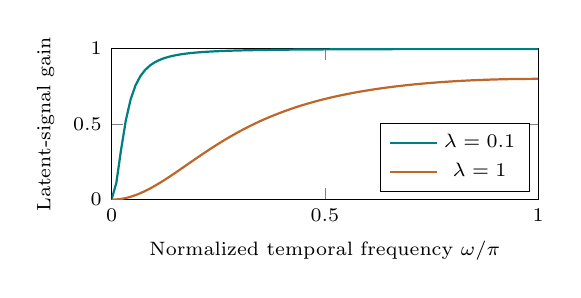
\begin{tikzpicture}
\begin{axis}[width=7cm,height=3.5cm,xmin=0,xmax=1,ymin=0,ymax=1,xtick={0,.5,1},ytick={0,.5,1},xlabel={Normalized temporal frequency $\omega/\pi$},ylabel={Latent-signal gain},label style={font=\scriptsize},tick label style={font=\scriptsize},legend style={font=\scriptsize,at={(.98,.05)},anchor=south east}]
% source: analytic continuous extension H(omega) in Ch. 4 eq:transfer_function; chosen illustrative lambda values.
\addplot[teal,thick,domain=0:1,samples=90]{4*sin(90*x)^2/(4*sin(90*x)^2+.01)};\addlegendentry{$\lambda=0.1$}
\addplot[amber,thick,domain=0:1,samples=90]{4*sin(90*x)^2/(4*sin(90*x)^2+1)};\addlegendentry{$\lambda=1$}
\end{axis}
\end{tikzpicture}
\column{.42\textwidth}
The baseline is removed.\par\medskip
Low temporal modes are attenuated most.\par\medskip
A unique estimate does not restore the missing physical baseline.\par\medskip
In the images: slow brightness drift fades; passing edges remain.
\end{columns}
% source detail: Ch. 4, lem:A\_spectrum, thm:frequency\_response. Curves: continuous extension.
\src{\dref{Lemma}{lem:A_spectrum}, \dref{Theorem}{thm:frequency_response}; cosine eigenbasis~\cite{strang1999discrete}. Curves: continuous extension.}
\talknote{Spectral interpretation; 75 seconds.}{The first-difference Gramian is the Neumann-chain Laplacian. Its constant eigenvector has eigenvalue zero. Expanding a noiseless latent signal in the eigenbasis turns reconstruction into multiplication by g/(g+lambda\textasciicircum{}2). These are latent-signal gains; the gain from noise in the difference observations is a different expression in the backup.}{The spectral decomposition is proved in Chapter 4 and reused here for stereo. The plotted smooth curves interpolate the finite-chain modal gains. Only omega\_k=pi k/n are exact finite-grid modes. This magnitude penalty attenuates low temporal frequencies most, whereas the temporal kernels may average rapid changes. Scene terms: slow brightness drift fades and passing edges remain, hence the edge-enhanced look.}
\end{frame}

\begin{frame}{MVSEC comparison with Antil--Sayre bilevel}
\begin{columns}[T]
\column{.41\textwidth}
\small MVSEC~\cite{MVSEC2018} indoor flying 2\par\medskip
% source: figures/reconstruction_evaluation/metadata.json (indoor_flying2_bump_05; reference and event-only panels).
\panel{.48}{figures/reconstruction_evaluation/reference.png}{Reference}
\hfill\panel{.48}{figures/reconstruction_evaluation/event_only_reconstruction.png}{Event only}
\column{.56\textwidth}
\small
\textbf{This chapter:} events only $\to$ activity weights $\Lam(dc)$ $\to$ fixed convex solve.\par\smallskip
\textbf{Antil--Sayre~\cite{HAntil_DSayre_2023a}:} events and frames $\to$ outer optimization over the blur-kernel parameter $z$.\par\medskip
\footnotesize
% source: https://arxiv.org/pdf/2302.02052, Sec. 3, Eqs. (3.1)--(3.3); Ch. 2 tab:bilevel_comp_indoor and tab:bilevel_comp_outdoor.
\begin{tabular}{lrrrr}\toprule
& \multicolumn{2}{c}{PSNR (dB)} & \multicolumn{2}{c}{CN}\\
Sequence & Bilevel & Events & Bilevel & Events\\\midrule
% source: Ch. 2 tab:bilevel_comp_indoor; reported PSNR and CN values.
Indoor & 15.37 & 10.85 & 39755 & 25.51\\
% source: Ch. 2 tab:bilevel_comp_outdoor; reported PSNR and CN values.
Outdoor & 8.41 & 8.71 & 39755 & 27.10\\\bottomrule
\end{tabular}\par\smallskip
{\scriptsize PSNR: similarity to a reference frame (dB). CN: condition number of each method's inner linear system.\par}
\end{columns}
% source detail: Antil--Sayre (2023), Sec. 3, Eqs. (3.1)--(3.3); Ch. 2, subsubsec:bilevel\_comparison, tab:bilevel\_comp\_indoor, tab:bilevel\_comp\_outdoor; images: MVSEC indoor flying 2, Ch. 2 saved release.
\src{\dref{Table}{tab:bilevel_comp_indoor} and \dref{Table}{tab:bilevel_comp_outdoor}. Antil--Sayre~\cite{HAntil_DSayre_2023a}, Sec. 3, Eqs. (3.1)--(3.3). Images: MVSEC indoor flying 2.}
\talknote{MVSEC evidence and the bilevel relation; about 2.5 minutes.}{Left: an MVSEC indoor frame and the event-only reconstruction; structure is recovered while the absolute brightness is the level the model selects. In Antil--Sayre, the outer variable $z_{xy}\in\R^{n_t}$ parameterizes the event-based blur kernel $g(z)$ that links each blurry frame to the latent image; it is not a regularization weight. Our Chapter 2 rule computes diagonal magnitude weights from event activity and then solves a fixed convex quadratic.}{PSNR compares with a reference frame, so it also scores the absolute brightness the model selects; the events constrain only changes. The methods receive different inputs, including intensity frames for the comparator, so the table is descriptive: frames buy PSNR indoors, while the event-only system is far better conditioned. Kernel comparisons are in the backup "Temporal evidence: structure without an absolute baseline".}
\end{frame}

\begin{frame}{Shared motion couples temporal profiles to one scene}
\centering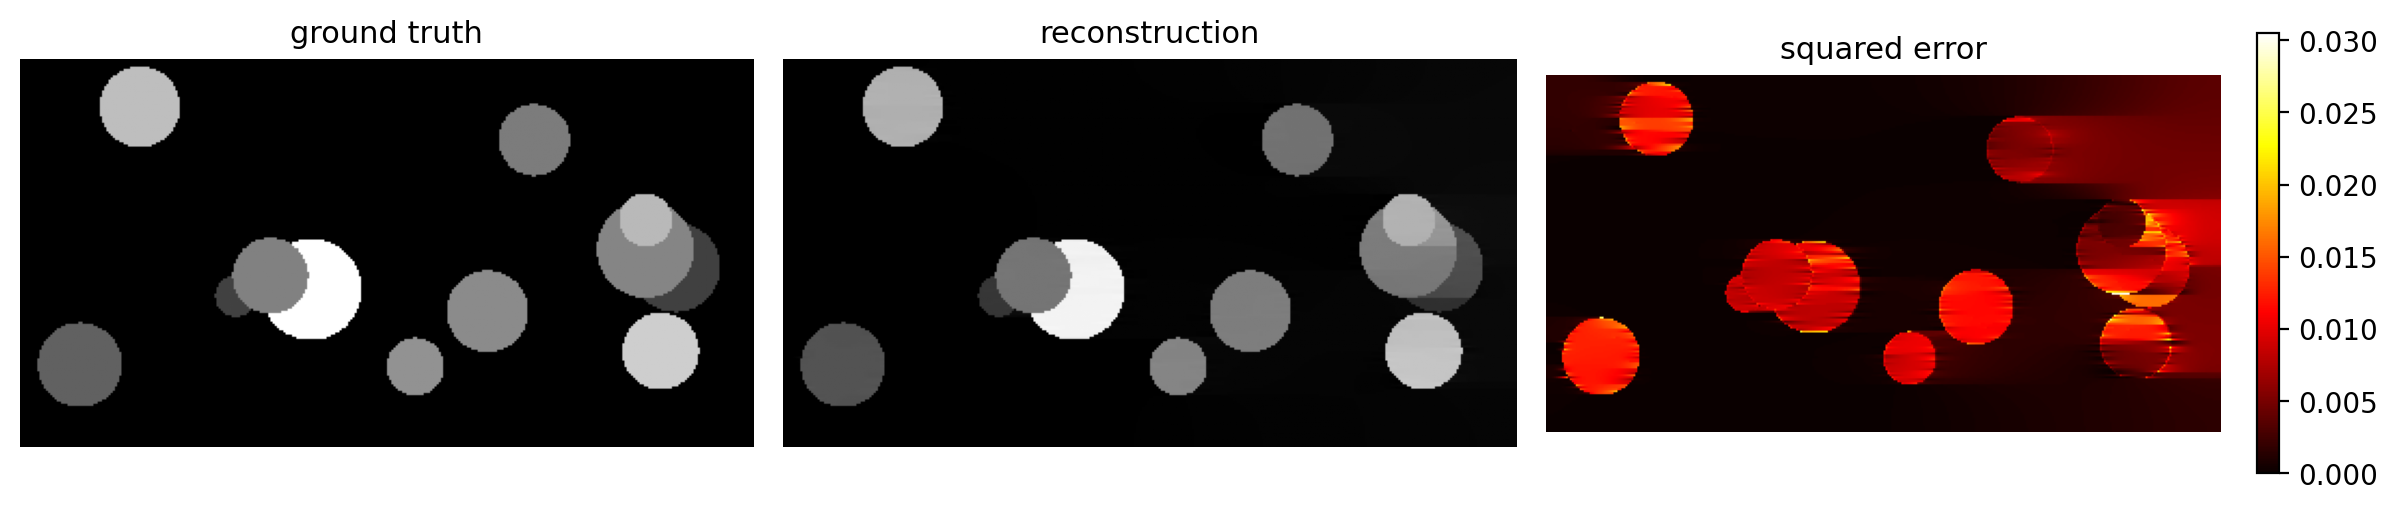
\includegraphics[width=\linewidth,height=2.55cm,keepaspectratio]{figures/sar_synthetic/disks_v2e.png}\par
% source: Ch. 2 sec:ch2_sar_bridge and fig:ch2_sar_synthetic; one-pixel horizontal translation per view, v2e events, smoothed-TV penalty.
{\scriptsize Simulated events (v2e~\cite{hu2021v2e}); the camera window shifts $1$\,px per view. Left: scene. Center: shared-scene estimate (smoothed-TV penalty). Right: squared error.\par}
\raggedright\vspace{1mm}
\begin{columns}[c]
\column{.50\textwidth}
\small\textbf{Chapter 2:} each pixel has its own temporal profile.\par\smallskip
\textbf{Shared scene:} known motion $P$ maps one static scene $\theta$ into every view.
\column{.46\textwidth}
% source: Ch. 2 eq:ch2_sar_forward.
\[\underbrace{B_{\rm SAR}}_{\text{scene-to-event operator}}=(A\otimes I)\,P.\]
\end{columns}
% source detail: Ch. 2, sec:ch2\_sar\_bridge, eq:ch2\_sar\_forward, prop:ch2\_sar\_solvability, fig:ch2\_sar\_synthetic.
\src{\dref{Figure}{fig:ch2_sar_synthetic}, \dref{Eq.}{eq:ch2_sar_forward}, \dref{Proposition}{prop:ch2_sar_solvability}; joint ESAR work~\cite{antil2026esareventbasedsyntheticaperture}; synthetic aperture~\cite{vaish2006synthetic}.}
\talknote{Shared-scene bridge; about 60 seconds. One idea: one scene, many views.}{Chapter 2 reconstructs independent pixel histories. In the joint ESAR work, $\theta$ is one static scene, the row-normalized footprint projections $P_k$ encode known motion and map it into each view, and $A$ differences consecutive views. The figure: twelve disks seen through a window translating one pixel per view; error concentrates along rows through the disks, the weakly constrained direction for horizontal motion. Chapter 3 then makes the motion itself the unknown.}{If asked for the algebra (Proposition 2.4.1): $\ker B_{\rm SAR}=\{\theta:P_{k+1}\theta=P_k\theta\}$ contains constants because $P_k\mathbf1=\mathbf1$; under translation, fields constant along the motion are weakly constrained. With unsquared ridge $\lambda>0$, $(B^\top B+\lambda I)\widehat\theta=B^\top b$ has a unique solution and $\norm{\delta\theta}\le\norm{B_{\rm SAR}}\norm{\delta b}/\lambda$. The figure uses a smoothed-TV penalty with the constant offset removed; the ridge result is the quadratic version of the same model. Other invariant modes depend on $P$ and the trajectory. JIF in Chapter 4 applies the same shared-unknown idea to two cameras.}
\end{frame}

\section{Dense optical flow}
\begin{frame}{The aperture problem: what a local view reveals}
\small An \textbf{aperture} is a restricted observation window: a small view of an edge~\cite{marr1981directional}.
\vspace{2mm}
\begin{columns}[T]
\column{.49\textwidth}\centering
\textbf{Through the windows}\par
\ifdefined\DefenseNotes
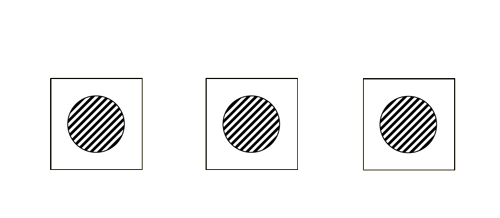
\includegraphics[width=\linewidth,height=2.65cm,keepaspectratio]{figures/aperture/masked.png}
\else
\ifdefined\DefensePresenter
\movie[loop]{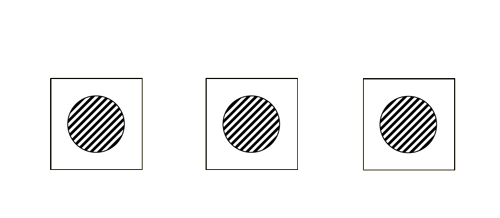
\includegraphics[width=\linewidth,height=2.3cm,keepaspectratio]{figures/aperture/masked.png}}{figures/aperture/app5-hide.mp4}
\else
\animategraphics[label=aperturemasked,width=\linewidth,height=2.3cm,keepaspectratio,poster=first,loop,controls={play,stop},buttonsize=2.5mm,buttonfg=0:0.498:0.514,method=widget,alttext={Masked stripes with ambiguous local motion}]{5}{figures/aperture/app5-hide/frame-}{0}{6}
\fi
\fi\par
{\footnotesize The visible stripe motions look the same.}\par\smallskip
\href{https://cdn.sinauer.com/wolfe4e/ch/08/act0802/app5-hide.gif}{\scriptsize\textcolor{teal}{Movie 5 source (GIF)}}
\column{.49\textwidth}\centering
\textbf{Reveal the full patterns}\par
\ifdefined\DefenseNotes
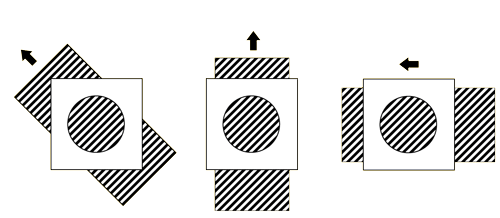
\includegraphics[width=\linewidth,height=2.65cm,keepaspectratio]{figures/aperture/revealed.png}
\else
\ifdefined\DefensePresenter
\movie[loop]{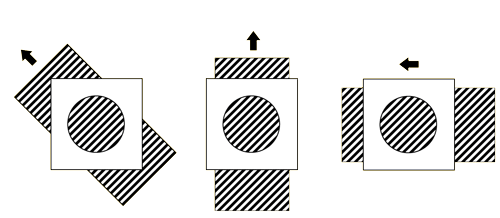
\includegraphics[width=\linewidth,height=2.3cm,keepaspectratio]{figures/aperture/revealed.png}}{figures/aperture/app6-show.mp4}
\else
\animategraphics[label=aperturerevealed,width=\linewidth,height=2.3cm,keepaspectratio,poster=first,loop,controls={play,stop},buttonsize=2.5mm,buttonfg=0:0.498:0.514,method=widget,alttext={Full stripe patterns with distinct translation directions}]{5}{figures/aperture/app6-show/frame-}{0}{6}
\fi
\fi\par
{\footnotesize The patterns translate in different directions.}\par\smallskip
\href{https://cdn.sinauer.com/wolfe4e/ch/08/act0802/app6-show.gif}{\scriptsize\textcolor{teal}{Movie 6 source (GIF)}}
\end{columns}
% source detail: Ch. 3, prop:time_surface and following aperture remark.
\vfill{\fontsize{6.5}{8}\selectfont\color{muted}Perceptual illustration: Wolfe et al., \emph{Sensation and Perception}, 4th ed., Sinauer \textcopyright\ 2015. \href{https://cdn.sinauer.com/wolfe4e/wa08.02.html\#Aperture}{\textcolor{teal}{Activity 8.2, Movies 5--6}}.\par Dissertation: \dref{Proposition}{prop:time_surface} and the following aperture discussion.\par}
\talknote{Define the aperture problem visually; about 90 seconds.}{Optical flow is apparent velocity in the image plane. An aperture simply means a restricted observation window. First look at the circular windows: the moving stripes look alike. Revealing the full patterns shows three different translation directions. A local straight edge tells us its speed perpendicular to the edge; motion along its tangent stays free. These publisher animations illustrate motion perception. They are conceptual demonstrations, rather than measured event-camera data.}{The two animations are embedded on this slide. Play the masked panel first using its forward-play control, then play the revealed panel; each loops at the original rate. First-frame posters preserve the visual comparison in static viewers and print. Use a PDF viewer with animation support and JavaScript enabled, as documented with the assets. Under steady illumination, different velocities with the same normal component produce the same local brightness changes and ideal events. Smoothness couples neighboring velocity estimates, while additional observed directions constrain the component left free by a single edge. Next, draw the same ambiguity for one edge and state the flow model in scene terms.}
\end{frame}

\begin{frame}{Motion introduces a new invisible direction}
\footnotesize
\vspace*{-3mm}
\begin{columns}[T]
\column{.47\textwidth}\centering
{\scriptsize\textbf{Image: one moving edge}}\par\smallskip
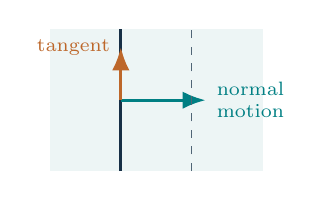
\begin{tikzpicture}[x=.45cm,y=.45cm,>=Latex]
\fill[soft] (0,0) rectangle (6,4);
\draw[ink,very thick] (2,0)--(2,4);
\draw[teal,very thick,->] (2,2)--(4.4,2) node[right,font=\scriptsize,align=left] {normal\\motion};
\draw[amber,very thick,->] (2,2)--(2,3.5) node[left,font=\scriptsize] {tangent};
\draw[muted,dashed] (4,0)--(4,4);
\end{tikzpicture}\par
{\scriptsize A straight edge reveals its normal speed.}
\column{.51\textwidth}\centering
{\scriptsize\textbf{Velocity: what the events allow}}\par\smallskip
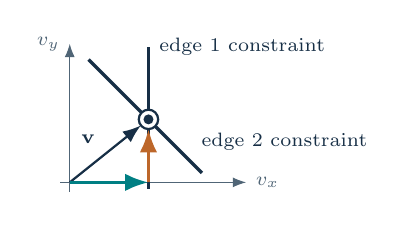
\begin{tikzpicture}[x=.4cm,y=.4cm,>=Latex]
\draw[muted,->] (-.3,0)--(5.6,0) node[right,font=\scriptsize] {$v_x$};
\draw[muted,->] (0,-.3)--(0,4.4) node[left,font=\scriptsize] {$v_y$};
\draw[ink,very thick] (2.5,-.2)--(2.5,4.3) node[right,font=\scriptsize] {edge 1 constraint};
\draw[ink,very thick] (.6,3.9)--(4.2,.3) node[pos=.9,above right,font=\scriptsize] {edge 2 constraint};
\draw[ink,thick,->,shorten >=3.5pt] (0,0)--(2.5,2) node[pos=.45,above left,font=\scriptsize] {$\mathbf v$};
\draw[teal,very thick,->] (0,0)--(2.5,0);
\draw[amber,very thick,->,shorten >=3.5pt] (2.5,0)--(2.5,2);
\draw[ink,fill=white,thick] (2.5,2) circle (3.5pt);
\fill[ink] (2.5,2) circle (1.8pt);
\end{tikzpicture}\par
{\scriptsize Edge 1 fixes the {\color{teal}normal} part; edge 2, if it shares the motion, fixes the {\color{amber}tangent} part.}
\end{columns}
\vspace{0mm}
\vspace{1mm}
{\scriptsize\textbf{Flow model:} events give each edge's normal speed; neighbors moving alike supply the rest.\par
\textbf{Requirement (main theorem):} edges in two orientations somewhere, so their constraint lines cross.\par}
% source detail: Ch. 3, prop:time_surface and aperture remark (normal-speed constraint); thm:unified_wellposedness (integrated identifiability). Velocity-space intersection of constraints: Adelson and Movshon (1982).
\ifdefined\DefenseCommittee\vspace{-1mm}{\fontsize{6.5}{8}\selectfont\color{muted}Intersection of constraints [Adelson \& Movshon 1982]. Dissertation: \dref{Proposition}{prop:time_surface}; requirement in \dref{Theorem}{thm:unified_wellposedness}.\par}\fi
\talknote{Flow model in scene terms; about two minutes.}{A pixel fires when its log brightness changes by the threshold, so firing times trace an image edge. Left: normal motion in teal, tangent in amber. Right, velocity space, no positions: each line is every velocity one edge's events allow. Teal is the normal part edge 1 measures; amber is the tangent part it leaves free. If edge 2 shares the motion, the lines cross at $\mathbf v$, teal plus amber. Shared motion is an assumption: non-parallel lines always cross, so for edges moving differently the crossing is wrong for both. Requirement: two orientations somewhere.}{With exact coefficients and one shared velocity, the constant field is the unique minimizer at any $\alpha$ and separation. Example: edge 1 vertical moving right at $s$, edge 2 with normal $(1,1)/\sqrt2$ stationary; estimate $(s,-s)$ everywhere. Time-surface coefficient at an edge: rank one, proportional to $\mathbf n\mathbf n^\top$; two non-parallel normals give a positive-definite sum, the integrated condition. Slide 19: stripes give one orientation inside, the checkerboard two. Intersection of constraints: Adelson and Movshon.}
\end{frame}

\begin{frame}{Three representations, one quadratic variational problem}
Rename the flow data matrix $\B$ to distinguish it from temporal $\A$:
\[E_{\B,b}(\vct)=\frac12\int_\Omega\bigl(\vct^\top\B\vct-2b^\top\vct\bigr)
+\frac{\alpha^2}{2}\int_\Omega|\nabla\vct|^2.\]
\renewcommand{\arraystretch}{1.2}
\begin{tabular}{llll}\toprule Representation & $\B$ & $b$ & Edge measurement from\\\midrule
Time surface & $\nabla\mathcal T\nabla\mathcal T^\top$ & $\nabla\mathcal T$ & crossing times\\
Voxel projection & $\nabla a\nabla a^\top$ & $-a_s\nabla a$ & transported event activity\\
Structure tensor & $\widetilde{\mathbf J}$ & $-\mathbf j_t$ & gradients pooled over a window\\\bottomrule
\end{tabular}
\par\smallskip
{\footnotesize In scene terms: $\B$ records which motion directions the edges measure, and how strongly; $b$ carries the measured values; the $\alpha$ term asks neighbors to move alike.\par}
% source detail: Ch. 3, thm:unified\_wellposedness and its three corollaries.
\src{\dref{Theorem}{thm:unified_wellposedness} and its three corollaries; data-plus-smoothness form~\cite{horn1981determining}.}
\talknote{Unification; 60 seconds.}{The energies agree with the representation-specific residual energies up to an overall positive factor and a constant independent of flow. The common space is H\textasciicircum{}1(Omega; R\textasciicircum{}2), and the Dirichlet term couples neighboring velocities.}{The notation B here is A\_data in the dissertation, and alpha is alpha\_smooth. The change avoids using A for two different operators on consecutive chapters. The common analysis is about fixed coefficients. A good mathematical estimator can still encode a poor representation of physical motion. Scene terms: $\B$ records which motion directions the edges measure and how strongly; $b$ the measured values.}
\end{frame}

\begin{frame}{The main flow theorem: global information controls constants}
\begin{block}{Unified well-posedness theorem}
Let $\Omega\subset\R^2$ be bounded, connected, and Lipschitz; $\alpha>0$.
Assume
\[\B\in L^\infty,\quad \B=\B^\top\succeq0\text{ a.e.},\quad b\in L^2,\qquad
\setlength{\fboxsep}{1.5pt}\boxed{\int_\Omega\B(\mathbf x)\,d\mathbf x\succ0}.\]
Then $E_{\B,b}$ has a unique minimizer in $H^1(\Omega;\R^2)$.
\end{block}
\vspace{1mm}
The integrated matrix must identify \textbf{every constant velocity direction}.\par
\small In scene terms: edges in two or more orientations somewhere, so their constraint lines cross; neighbors supply the motion where $\B=0$.
% source detail: Ch. 3, thm:unified\_wellposedness, eq:integrated\_identifiability.
\src{\dref{Theorem}{thm:unified_wellposedness}, \dref{Eq.}{eq:integrated_identifiability}; classical quadratic-flow theory~\cite{weickert2001theoretical}.}
\talknote{Central theorem; 90 seconds.}{Classical quadratic optical flow already has well-posedness theory, including Weickert and Schn\"orr. The contribution here is one analysis for three event-derived coefficient constructions, with explicit identifiability and perturbation hypotheses. Read the hypotheses and interpret each. Connectedness makes the kernel of the gradient consist of global constants. The positive regularization coefficient controls spatial variation. Bounded data curvature and L2 forcing make the weak forms bounded. Positive definiteness of the integrated B controls constant fields that smoothness cannot see.}{B may vanish on open subsets while its integral remains positive definite. In these observation models the residual forcing b also vanishes there, and smoothness propagates information from observed regions. For time surfaces, no nonzero vector can be perpendicular to all measured gradients almost everywhere. The condition need not hold pointwise. Scene terms: edges in at least two orientations somewhere in the image. The one hypothesis the scene must supply; if it fails, a uniform slide along the null direction leaves the energy unchanged (Backup 35). It is checked on represented data, including smoothing artifacts at never-fired pixels. Accuracy rests on slide 16's shared-motion assumption (measured on slide 19).}
\end{frame}

\begin{frame}{Known-motion examples make the aperture problem visible}
\centering\small
\begin{tabular}{lccc}
 & Ground truth & Voxel & Structure tensor\\
\rotatebox{90}{Stripes}\! & 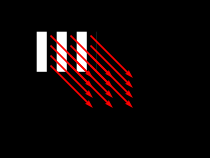
\includegraphics[width=2.75cm]{figures/ch3_quivers_consistent/v2e_stripes_f0022/crop/gt.png}&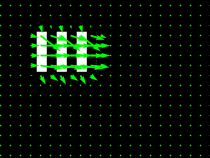
\includegraphics[width=2.75cm]{figures/ch3_quivers_consistent/v2e_stripes_f0022/crop/vox.png}&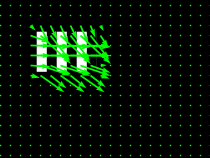
\includegraphics[width=2.75cm]{figures/ch3_quivers_consistent/v2e_stripes_f0022/crop/vox_struct.png}\\
\rotatebox{90}{Checker}\! & 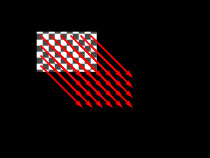
\includegraphics[width=2.75cm]{figures/ch3_quivers_consistent/v2e_checker_f0022/crop/gt.png}&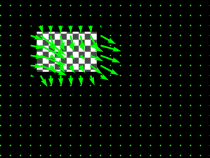
\includegraphics[width=2.75cm]{figures/ch3_quivers_consistent/v2e_checker_f0022/crop/vox.png}&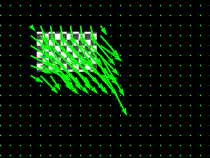
\includegraphics[width=2.75cm]{figures/ch3_quivers_consistent/v2e_checker_f0022/crop/vox_struct.png}\\
\end{tabular}
% source detail: Ch. 3, fig:ch3\_quiver\_v2e; v2e simulation, same window and arrow scale.
\src{\dref{Figure}{fig:ch3_quiver_v2e}; v2e~\cite{hu2021v2e} simulation, same window and arrow scale.}
\talknote{Visual evidence; 60 seconds.}{The object translates diagonally. Red arrows show the ground truth and green arrows the estimates, at the common scale retained from the dissertation's panels. Vertical stripe interiors provide mainly horizontal gradients. The checkerboard provides gradient information in both spatial directions. Object boundaries can supply additional information even in the stripe scene.}{These are selected illustrative windows, not a cross-dataset method ranking. The full figure also includes time surface and other variants; its reported TS AEE equals the zero-field baseline at the reported precision. The output does not diagnose which hypothesis or extraction step fails, so do not assign a cause.}
\end{frame}

\section{Stereo depth}
\begin{frame}{Stereo depth: competitive accuracy, most scored points}
\begin{columns}[c]
\column{.38\textwidth}\centering
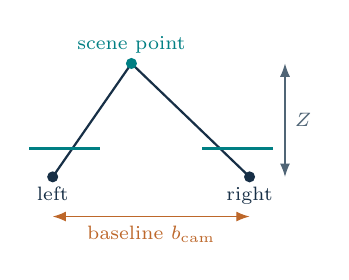
\begin{tikzpicture}[x=.5cm,y=.36cm,>=Latex]
\coordinate (L) at (0,0);\coordinate (R) at (5,0);\coordinate (P) at (2,4);
\draw[ink,thick] (L)--(P)--(R);\fill[teal] (P) circle(2pt) node[above,font=\scriptsize] {scene point};
\draw[teal,thick] (-.6,1)--(1.2,1);\draw[teal,thick] (3.8,1)--(5.6,1);
\fill[ink] (L) circle(2pt) node[below,font=\scriptsize] {left};\fill[ink] (R) circle(2pt) node[below,font=\scriptsize] {right};
\draw[<->,amber] (0,-1.4)--(5,-1.4) node[midway,below,font=\scriptsize] {baseline $b_{\rm cam}$};
\draw[<->,muted] (5.9,0)--(5.9,4) node[midway,right,font=\scriptsize] {$Z$};
\end{tikzpicture}
\column{.58\textwidth}
\small
\[Z=\frac{f_{\rm cam}b_{\rm cam}}{d},\qquad d=x_L-x_R>0.\]
Each candidate $d$ pairs the two views, and one shared temporal profile is fitted to both. For fixed $d$ and frozen weights the inner solve is unique.
\end{columns}
\vspace{2mm}
\centering\footnotesize
\begin{tabular}{lrrrrrr}
\toprule & \multicolumn{4}{c}{Mean depth error (cm) $\downarrow$}&log RMSE&Scored\\
Method & Fl1&Fl2&Fl3&Fl4&$\times100\;\downarrow$&points (M)\\\midrule
% source: appendix_bodies/ch4_protocol.tex tab:unified_benchmark, wls row (mean error, log RMSE x100, #Pts).
\textbf{WLS (ours)}&73.83&\textbf{58.35}&70.33&59.24&\textbf{44.54}&\textbf{2.66}\\
% source: appendix_bodies/ch4_protocol.tex tab:unified_benchmark, Piatkowska row.
Piatkowska adaptation~\cite{piatkowska2017}&\textbf{67.96}&58.75&\textbf{68.88}&\textbf{54.63}&44.72&1.20\\\bottomrule
\end{tabular}\par\smallskip
% source: appendix_bodies/ch4_protocol.tex tab:metrics, per-method population; depth band [0.5,8] m; tab:unified_benchmark: 2.66M is the largest of the five methods.
{\scriptsize MVSEC indoor flying 1--4; each method scored on its own estimates in $[0.5,8]$\,m. Three more methods in the backup table.\par}
% source detail: Ch. 4, sec:solution, eq:depth\_conversion, thm:weighted\_spd; App., tab:unified\_benchmark, tab:metrics. Geometry is schematic.
\src{\dref{Section}{sec:solution}, \dref{Eq.}{eq:depth_conversion}, \dref{Theorem}{thm:weighted_spd}; \dref{Table}{tab:unified_benchmark}; MVSEC~\cite{MVSEC2018}. Geometry is schematic.}
\talknote{Stereo summary; about 3 minutes.}{Rectification places corresponding rays on the same image row; disparity is the horizontal shift and similar triangles give depth. At each candidate disparity, two softly coupled temporal profiles are solved; with frozen positive weights the Hessian is at least $\lambda_{\min}^2\mathbf I$, the Chapter 2 argument with one more nonnegative term. The benchmark uses the full WLS method: weight updates, cost aggregation, and candidate selection.}{WLS leads on Flying 2 and log RMSE; the Piatkowska adaptation leads on Flying 1, 3, and 4 by 5.9, 1.5, and 4.6 cm; WLS scores 2.66M points, the most of the five methods and 2.2 times Piatkowska's. Each method is scored on its own valid pixels, so read accuracy together with coverage. Correspondence questions go to the Chapter 4 backups.}
\end{frame}

\section{Contributions and next questions}
\begin{frame}{Research opportunities}
\small
\begin{columns}[T]
\column{.24\textwidth}
\begin{block}{Sensor modeling}
Measure the error terms of slide~9 on real sensors; the stability bounds turn them into estimate bounds.
\end{block}
\column{.24\textwidth}
\begin{block}{Learned weights}
Learn $\Lam$ in an outer problem [Antil--Di--Khatri 2020]; for $\Lam\succ0$, $\mathbf f^*(\Lam)$ is smooth.
\end{block}
\column{.24\textwidth}
\begin{block}{Shared scenes}
Find the motion-invariant modes of $B_{\rm SAR}$ for a trajectory (ESAR~\cite{antil2026esareventbasedsyntheticaperture}); apply to orbital streams.
\end{block}
\column{.24\textwidth}
\begin{block}{Edge hardware}
Update only pixels with events; measure time and power on a Raspberry Pi~5 and edge sensors.
\end{block}
\end{columns}
% source detail: Ch. 2, subsubsec:physical, thm:uniqueness, prop:ch2\_sar\_solvability; Ch. 3, eq:abstract\_stability; Ch. 5, Future Directions. External: Antil, Di, Khatri, Inverse Problems 36 (2020) 064001. Edge implementation: monocular_reconstruction/python/edge.
\src{\dref{Chapter}{ch:discussion_conclusion}, Future Directions; physical connection (\drefpage{subsubsec:physical}); \dref{Proposition}{prop:ch2_sar_solvability}. External paper cited above.}
\talknote{Future research; about 90 seconds.}{Sensor modeling: the identity on slide 9 names the error terms; measuring them on a real sensor gives the input the stability bounds need. The GMU Neuromorphic Imaging and Digital Twins Lab (AFOSR DURIP) makes those controlled acquisitions possible. Learned regularization: $\mathbf f^*(\Lam)=(\A^\top\A+\Lam^2)^{-1}\A^\top\mathbf y$ is rational and hence smooth in $\Lam$ on the positive orthant, which a bilevel analysis needs from its lower level.}{Shared scene: the ESAR null space contains constants and any other motion-invariant scene modes. Edge implementation: the streaming form updates each pixel in constant time; updating only pixels with events, and timing the method on a Raspberry Pi 5 with a power meter, are the next steps. Then go to the closing slide.}
\end{frame}

\begin{frame}{What the data constrain and what the models prove}
\footnotesize\renewcommand{\arraystretch}{1.05}
\begin{tabular}{>{\raggedright\arraybackslash}p{2.6cm}>{\raggedright\arraybackslash}p{4.4cm}>{\raggedright\arraybackslash}p{5.9cm}}\toprule
Problem & What the observations constrain & What the mathematical model establishes\\\midrule
Temporal reconstruction & Represented brightness increments & Unique regularized history for each fixed positive weight matrix, with perturbation bounds\\
Optical flow & Event-derived directional motion constraints & Unique $H^1$ minimizer under integrated identifiability\\
Stereo depth & Paired temporal event-feature observations & Unique frozen-weight inner solve; the disparity comes from a separate comparison of candidates\\\bottomrule
\end{tabular}
\takeaway{Under the stated hypotheses, regularization makes each estimator determinate; accuracy also depends on the representation.}
% source detail: Ch. 2 thm:uniqueness; Ch. 3 thm:unified\_wellposedness; Ch. 4 thm:weighted\_spd; Ch. 5, tab:contribution\_matrix.
\src{\dref{Theorem}{thm:uniqueness}, \dref{Theorem}{thm:unified_wellposedness}, \dref{Theorem}{thm:weighted_spd}; \dref{Table}{tab:contribution_matrix}.}
{\small\textcolor{teal}{\textbf{Which directions do the observations control, and which are selected by the model?}}\par\hfill Thank you.\par}
\talknote{Contributions and close; about 90 seconds.}{Read across each row: what the events constrain, then what the model proves. If asked about recomputed weights: Backup 65 (page 98) gives a local Lipschitz bound beyond the dissertation. The temporal null mode is selected by a penalty. Spatial smoothness and integrated directional data make the flow energy coercive. Stereo has a well-posed latent solve at each candidate; selecting the candidate is a separate decision.}{Close by returning to the common question, then stop for committee questions. Position the originality accurately: the functional-analytic tools are classical; the dissertation organizes event-derived models under explicit hypotheses and derives the coupling, conditioning, bias, and selection consequences. If asked about results beyond the table: contrast-maximization existence, graph convergence of the discrete flow, selection margins, and IRLS fixed-point and contraction results are in the backups and in Ch.\ 5, Table on the contribution matrix.}
\end{frame}

\appendix
\backuptrue
\section{Discussion and additional proofs}
% Discussion slides are outside the timed core. Their source labels name the dissertation.
\begin{frame}{Discussion guide}
\footnotesize
\begin{columns}[T]
\column{.48\textwidth}
\textbf{Observation and temporal inversion}
\begin{itemize}
\item Minimal uniqueness condition / gauge
\item Measure-valued continuous-time limit
\item Signal gain versus noise gain
\item Kernel comparison on indoor and outdoor data
\end{itemize}
\textbf{Flow analysis}
\begin{itemize}
\item Weak Euler equation and boundary condition
\item Exact block-Jacobi spectral argument
\item Anisotropy and ellipticity
\item Regression design and projection mismatch
\end{itemize}
\column{.48\textwidth}
\textbf{Stereo analysis}
\begin{itemize}
\item Mean-zero conditioning
\item Cost ellipsoid and observation perturbations
\item IRLS contraction proof
\item Fixed points versus likelihood stationarity
\item Implemented scoring and aggregation
\end{itemize}
\textbf{Evidence and interpretation}
\begin{itemize}
\item Depth evaluation, coverage, and selection
\item What is contributed by the dissertation?
\item Literature anchors and source map
\end{itemize}
\end{columns}
\talknote{Use as an appendix index.}{The following slides support questions rather than extend the planned talk. PDF section bookmarks and the source-map file make it possible to find their manuscript origins.}{Each discussion slide has notes that give the proof mechanism or a suggested concise answer.}
\end{frame}



\begin{frame}{Must every temporal penalty entry be positive?}
For arbitrary $\Lam$, the exact algebraic criterion is
\[\A^\top\A+\Lam^\top\Lam\succ0
\quad\Longleftrightarrow\quad\ker\A\cap\ker\Lam=\{0\}.\]
\begin{block}{Why?}
The quadratic form vanishes precisely when both $\A\mathbf z=0$ and $\Lam\mathbf z=0$.
\end{block}
On a connected first-difference chain, $\ker\A=\operatorname{span}\{\mathbf1\}$.
\begin{itemize}
\item A single nonzero diagonal penalty entry removes that constant mode.
\item Fixing one reference value or imposing zero mean also removes it.
\end{itemize}
\takeaway{A gauge resolves the mathematical ambiguity; a measured reference would add physical information.}
\src{Ch. 2, lem:nullspace; Ch. 4, discussion following lem:A\_spectrum.}
\talknote{Question: why use a full positive diagonal?}{The main theorem's positive diagonal is a strong sufficient hypothesis with an immediate quantitative lower bound. It is not necessary for definiteness. The kernel-intersection argument shows the minimal condition. A one-point anchoring penalty gives definiteness, but its eigenvalue bound is not the same as lambda\_min squared when other diagonal entries are zero.}{An explicit zero-mean parameterization can avoid penalizing the unobserved offset. It changes the estimator: the original magnitude penalty also attenuates nonconstant modes and controls noise. Choosing a gauge alone never recovers an unmeasured absolute brightness baseline.}
\end{frame}

\begin{frame}{The event measure has a jump primitive}
At one pixel, set $\mu=\sum_jp_j\delta_{s_j}$, and choose a consistent right-continuous primitive
\[g(t)=f_0+\mu((t_0,t]),\qquad g(b)-g(a)=\mu((a,b]).\]
For a standard smooth compactly supported unit-mass kernel,
\[e_h=\mu*\phi_h,\qquad g_h(t)=f_0+\int_{t_0}^t e_h(\xi)\,d\xi.\]
For finitely many interior events, $g_h\to g$ in $L^1$ as $h\downarrow0$.
\begin{itemize}
\item $g$ belongs to $BV$; a nonzero interior jump prevents $g\in H^1$.
\item The displayed $g$ is an unregularized cumulative-event surrogate.
\end{itemize}
\takeaway{Keep interval conventions consistent and use increments, rather than an unscaled derivative, in $\A\mathbf f\approx\mathbf y$.}
\src{Ch. 2, subsubsec:ode; endpoint convention made explicit here.}
\talknote{Question: what is the continuous-time problem?}{A finite atomic measure has a bounded-variation cumulative primitive. For a nonzero interior atom its derivative is singular, so it cannot have an L2 weak derivative and is not H1. With finite standard bounded kernels of positive width, the smoothed driver is L2 and its primitive is H1. Arbitrary L1 alone would only guarantee W1,1.}{The bin convention (a,b] here matches the right-continuous process exactly. Alternative half-open bins are valid with a compatible representative or an explicit no-boundary-events assumption. The difference quotient is the integrated event increment divided by the time step; the discrete A in the presentation computes increments. The limit is not a convergence theorem for the regularized minimizer as the penalty and grid vary.}
\end{frame}

\begin{frame}{Latent-signal gain and observation-noise gain are different}
For the unweighted monocular model with scalar $\lambda>0$,
\[\mathbf f^*=(\A^\top\A+\lambda^2\mathbf I)^{-1}\A^\top\mathbf y.\]
\renewcommand{\arraystretch}{1.45}
\begin{tabular}{lll}\toprule Input & Output modal gain & Interpretation\\\midrule
Latent signal & $g_k/(g_k+\lambda^2)$ & Low modes attenuated most\\
Difference observation & $\sqrt{g_k}/(g_k+\lambda^2)$ & Noise amplitude transfer\\
White difference noise & $\sigma^2g_k/(g_k+\lambda^2)^2$ & Reconstructed modal variance\\\bottomrule
\end{tabular}
\vspace{3mm}
% source: Ch. 4 prop:noise_gain; max_{g>=0} g/(g+lambda^2)^2=1/(4lambda^2), derivative vanishes at g=lambda^2.
\[\max_{g\ge0}\frac{g}{(g+\lambda^2)^2}=\frac1{4\lambda^2}.\]
\src{Ch. 4, thm:frequency\_response, prop:noise\_gain.}
\talknote{Question: what kind of filter is this?}{Take the singular-value decomposition A=U Sigma V\textasciicircum{}T. The reconstruction operator maps left singular modes of y to right singular modes with amplitude sqrt(g)/(g+lambda squared). Multiplying by A for noiseless y=A f\_true yields the latent-signal gain g/(g+lambda squared). For white independent observation noise the output covariance diagonalizes in the same right modes and its modal variance is sigma squared times the squared observation gain.}{Differentiate g/(g+a)\textasciicircum{}2 with a=lambda squared: the derivative has sign a-g, so the continuous maximum is 1/(4a) at g=a. The discrete finite-chain maximum may be smaller because its available eigenvalues need not contain a. These formulas do not carry over unchanged to arbitrary diagonal penalties or unequal adaptive stereo weights.}
\end{frame}

\begin{frame}{Kernel performance depends on the scene and adaptive weights}
\small\renewcommand{\arraystretch}{1.2}
\begin{center}\begin{tabular}{lrrrr}\toprule
&\multicolumn{2}{c}{MVSEC indoor}&\multicolumn{2}{c}{MVSEC outdoor}\\
Kernel&PSNR&CN&PSNR&CN\\\midrule
% source: Ch. 2 tab:bump_avg_indoor and tab:bump_avg_outdoor, B-spline rows.
B-spline&8.86&22.16&6.72&97.92\\
% source: Ch. 2 tab:bump_avg_indoor and tab:bump_avg_outdoor, Delta rows.
Delta&7.70&1375.75&7.97&53.34\\
% source: Ch. 2 tab:bump_avg_indoor and tab:bump_avg_outdoor, Gaussian rows.
Gaussian&8.84&20.22&6.81&98.90\\
% source: Ch. 2 tab:bump_avg_indoor and tab:bump_avg_outdoor, Rectangular rows.
Rectangular&8.24&423.59&7.20&148.33\\\bottomrule
\end{tabular}\end{center}
\begin{itemize}
\item The temporal operator stays the same; represented data and adaptive penalties change.
\item Better conditioning is not the same as smaller reconstruction bias.
\item Reference-image scores do not identify an absolute intensity baseline from events.
\end{itemize}
\src{Ch. 2, tab:bump\_avg\_indoor, tab:bump\_avg\_outdoor.}
\talknote{Question: why does a smoothing kernel change conditioning?}{The matrix K=A\textasciicircum{}T A+Lambda\textasciicircum{}T Lambda does not directly contain the bump kernel. However Lambda is computed adaptively from represented observations. Changing aggregation can change those weights, hence the numerical matrix. The observed condition-number difference cannot be attributed to smoothing of a fixed operator alone.}{The table is copied from the dissertation, with aggregate labels retained. Its outdoor ordering shows why it would be excessive to claim one kernel is uniformly best. The positivity theorem is independent of the empirical ranking and gives only a sufficient worst-case bound, not a causal explanation of every numerical comparison.}
\end{frame}

\begin{frame}{The weak equation supplies the natural boundary condition}
For every $\boldsymbol\eta\in H^1(\Omega;\R^2)$,
\[\int_\Omega(\B\vct^*-b)\cdot\boldsymbol\eta
+\alpha^2\int_\Omega\nabla\vct^*:\nabla\boldsymbol\eta=0.\]
Interior tests give the distributional equation
\[-\alpha^2\Delta\vct^*+\B\vct^*=b.\]
Since the coefficients imply $\Delta\vct^*\in L^2$, Green's identity gives
\[\partial_n\vct^*=0\quad\text{in }H^{-1/2}(\partial\Omega;\R^2).\]
\takeaway{The theorem uses $H^1$ fields and weak traces, without claiming a classical solution on a Lipschitz domain.}
\src{Ch. 3, time-surface, voxel and structure-tensor Euler--Lagrange theorems.}
\talknote{Question: which boundary condition is imposed?}{The energy is minimized over the unrestricted H1 space, not H1\_0, so natural Neumann conditions emerge from the first variation. Compactly supported smooth tests first give the interior equation. B v and b are in L2, hence the distributional Laplacian is L2, so the gradient has a weak normal trace.}{Returning to arbitrary H1 tests, generalized Green's identity leaves a boundary pairing with their traces. Surjectivity of the trace map makes the normal trace zero. The anisotropic form replaces grad by D grad and yields a conormal condition n\textasciicircum{}T D grad v=0. No differentiability of D is needed for its weak formulation.}
\end{frame}

\begin{frame}{Why block-Jacobi converges for this graph model}
Absorb $q_i$ into $\widehat\B_i=q_i\B_i\succeq0$. Set
\[D_i=\alpha^2d_i\mathbf I+\widehat\B_i,\qquad R_{ij}=\alpha^2w_{ij}\mathbf I.\]
For symmetric nonnegative edge weights,
\[\mathbf z^\top(D\mp R)\mathbf z=\sum_i\mathbf z_i^\top\widehat\B_i\mathbf z_i
+\alpha^2\sum_{\{i,j\}}w_{ij}\norm{\mathbf z_i\mp\mathbf z_j}^2.\]
Connectedness and $\sum_i\widehat\B_i\succ0$ eliminate both constant and alternating constant zero modes (the latter on bipartite graphs).
\[D-R\succ0,\quad D+R\succ0\quad\Rightarrow\quad
-\mathbf I\prec D^{-1/2}RD^{-1/2}\prec\mathbf I.\]
\takeaway{The Jacobi iteration matrix is similar to a symmetric matrix with spectral radius strictly below one.}
\src{Ch. 3, extension of thm:convergence and cor:convergence\_psd\_blocks by absorbing $q_i$ into $\widehat\B_i$. $\alpha>0$, $d_i>0$.}
\talknote{Question: why does SPD suffice here for Jacobi?}{It does not suffice in general. The special graph form proves more. For D-R, a zero edge sum forces equality of neighbors, so all node vectors equal a constant. For D+R, it forces opposite vectors on every edge; on a bipartite graph they are alternating copies of one constant vector, while an odd cycle forces zero. The sampled PSD data blocks eliminate any nonzero constant or alternating constant.}{D is SPD because alpha and each degree are positive. Conjugate D plus or minus R by D\textasciicircum{}{-1/2}; the two positivity statements bound the symmetric spectrum between minus and plus one. D\textasciicircum{}{-1}R is similar to it, hence its spectral radius is below one and repeated simultaneous sweeps converge. An event-triggered partial-update schedule is a separate question.}
\end{frame}

\begin{frame}{Anisotropy needs a uniform ellipticity floor}
For the normalized Nagel--Enkelmann tensor, write $g=\nabla\rho_{\rm evt}$ and $\gamma_{\rm NE}>0$:
% source: Ch. 3 eq:ne_tensor; this is the normalized variant used in the dissertation.
\[\mathbf D=\frac{g^\perp(g^\perp)^\top+\gamma_{\rm NE}^2\mathbf I}{|g|^2+\gamma_{\rm NE}^2}.
\]
Its tangent and normal eigenvalues are
\[1,\qquad\frac{\gamma_{\rm NE}^2}{|g|^2+\gamma_{\rm NE}^2}.\]
If $g\in L^\infty$,
\[\theta\mathbf I\preceq\mathbf D\preceq\mathbf I,\qquad
\theta=\frac{\gamma_{\rm NE}^2}{\norm{g}_{L^\infty}^2+\gamma_{\rm NE}^2}>0.\]
\takeaway{Diffusion across event-density edges is reduced, while coercivity survives with $\alpha^2\theta$.}
\src{Ch. 3, normalized variant of eq:ne\_tensor, lem:ne\_elliptic, cor:structure\_wellposedness.}
\talknote{Question: can an adaptive diffusion tensor retain well-posedness?}{For a fixed, bounded, symmetric tensor with a common strictly positive lower eigenvalue bound, the Poincare/coercivity argument survives. Merely saying positive definite at each point is insufficient if eigenvalues approach zero. The normalized Nagel--Enkelmann form provides an explicit uniform floor when the density gradient is bounded.}{The tensor reduces penalties on normal-direction flow variations and preserves the tangent-direction penalty. If it is recomputed after data perturbation, stability includes ||D\_1-D\_2||\_infty. Event-density edges need not coincide with motion boundaries. The CM tensor alpha\_ani squared J plus epsilon I has the opposite directional effect: it increases the normal-direction penalty.}
\end{frame}

\begin{frame}{A variable diffusion tensor must stay inside the divergence}
For differentiable $\mathbf D$,
\begin{align*}
\nabla\!\cdot(\mathbf D\nabla u)
&=D_{11}u_{xx}+2D_{12}u_{xy}+D_{22}u_{yy}\\
&\quad+(\partial_xD_{11}+\partial_yD_{12})u_x
+(\partial_xD_{12}+\partial_yD_{22})u_y.
\end{align*}
% source: Ch. 3 eq:aniso_divergence_expansion and subsequent counterexample.
Take $\rho_{\rm evt}=x^2/2$, $\gamma_{\rm NE}=1$, and $u=x$:
\[\mathbf D=\operatorname{diag}\!\left(\frac1{1+x^2},1\right),\qquad
\nabla\!\cdot(\mathbf D\nabla u)=\frac{-2x}{(1+x^2)^2}\not\equiv0.\]
All second derivatives of $u$ vanish, so the principal part alone gives the wrong answer.
\src{Ch. 3, rem:aniso\_discretization.}
\talknote{Question: can you just replace the Laplacian by a tensor-weighted Hessian?}{Only for a constant tensor or when its coefficient-derivative contributions vanish. With a variable tensor the product rule supplies first-order terms. The affine test field exposes their importance particularly clearly, because its Hessian vanishes identically while its divergence-form diffusion does not.}{For merely L-infinity D, those classical coefficient derivatives may not exist. Keep the weak form integral grad eta transpose D grad u; it requires no derivative of D. A flux-consistent discretization should approximate that divergence form rather than drop terms without an error analysis.}
\end{frame}

\begin{frame}{The regression radius formula is a heuristic}
For full disks on a square lattice of spacing $h$, with $r/h$ large,
% source: Ch. 3 prop:ts_regression_bound(iv), eq:ts_radius_surrogate.
\[Q\sim\frac{\pi r^4}{4h^2}\mathbf I,\qquad
U_h(r)=\frac4{81}L_H^2r^4+\frac8\pi\sigma^2h^2r^{-4}.\]
The minimum of this leading expression, when all parameters are positive, is
% source: Ch. 3 radius-selection paragraph; r*^8=(162/pi) sigma^2 h^2 / L_H^2.
\[r^*=(162/\pi)^{1/8}(\sigma h/L_H)^{1/4}.\]
\begin{itemize}
\item The full disk must lie in a region with the asserted smoothness bound.
\item $U_h$ is an asymptotic expression for the finite-design bound, not itself a proved bound on every discrete MSE.
\item Affine time surfaces have zero curvature bias; this model supplies no finite balancing radius there.
\end{itemize}
\src{Ch. 3, prop:ts\_regression\_bound and Radius selection as a heuristic.}
\talknote{Question: is your radius choice optimal?}{Differentiate the positive leading bias-squared plus variance expression, which scales as A r\textasciicircum{}4 + B r\textasciicircum{}{-4}. Its stationary radius obeys r\textasciicircum{}8=B/A. The resulting scaling is a guide to how timestamp noise, lattice spacing, and curvature interact.}{The exact finite-design bound uses lattice sums. The asymptotic error has no stated sign, so the leading surrogate is not automatically an upper bound. The formula also requires positive curvature Lipschitz bound and noise, a large radius in lattice units, and inclusion in the smoothness neighborhood. Boundary truncation or sparse event support can destroy central symmetry and alter the bias.}
\end{frame}

\begin{frame}{Uniform projection and OLS slope need not be transport partners}
The continuous OLS temporal slope over $[s,s+T]$ is
\[\widehat\beta=\int_s^{s+T}w_s(t)V_t(t)\,dt,\qquad
w_s(t)=\frac{6(t-s)(s+T-t)}{T^3}.\]
Its transport-consistent spatial partner is the same $w_s$-weighted projection.
Pairing it with a uniform projection gives residual
\[\vct\cdot\nabla\int_s^{s+T}(T^{-1}-w_s(t))V(\mathbf x,t)\,dt.\]
% source: Ch. 3 derivative-operator qualifications, transported cubic counterexample.
For $V(x,t)=(2+x-t)^3$, $\vct=(1,0)$, $s=0$, $T=1$, this residual is $1/10$.
\takeaway{Well-posedness of a fixed-coefficient energy does not certify derivative consistency.}
\src{Ch. 3, subsec:vox\_projection, consistent derivative-operator discussion.}
\talknote{Question: why distinguish the implementation from exact transport?}{Integration by parts in the OLS slope formula yields the parabolic weight w\_s on the temporal derivative. Integrating the transport equation with that weight gives a correspondingly weighted spatial gradient. Using a uniform mean on one side and an OLS slope on the other generally gives a residual mismatch.}{Uniform and OLS weights share zeroth and first temporal moments, so transported polynomials through degree two have zero mismatch. A difference between their averages for a quadratic profile does not prove a nonzero transport residual. The cubic example supplies an actual derivative mismatch. This is a representation-coefficient error that the abstract stability theorem can address if its norm and identifiability hypotheses are controlled.}
\end{frame}

\begin{frame}{Mean-zero conditioning removes the unobserved mode}
In the unweighted scalar model, restrict to
\[\mathcal V_0=\{(\fL,\fR):\mathbf1^\top\fL=\mathbf1^\top\fR=0\}.\]
The sum--difference transform preserves this space. Its remaining eigenvalues are
% source: Ch. 4 cor:mean_zero_conditioning; g_k=4 sin^2(pi k/(2n)), k=1,...,n-1.
\[g_k+\lambda^2,\qquad g_k+\lambda^2+2\gamma,\qquad k=1,\ldots,n-1.\]
Thus
% source: Ch. 4 cor:mean_zero_conditioning, eq:kappa_mean_zero.
\[\kappa_2(\M|_{\mathcal V_0})=\frac{g_{\max}+\lambda^2+2\gamma}{g_1+\lambda^2}
\le\frac{g_{\max}+2\gamma}{g_1},\qquad g_1=4\sin^2\frac\pi{2n}.\]
\takeaway{The restriction is SPD even at $\lambda=0$. The uniform-in-$\lambda$ bound depends on the temporal grid; full-space perturbations remain different.}
\src{Ch. 4, cor:mean\_zero\_conditioning; prop:weighted\_conditioning (notes).}
% source: Ch. 4 prop:weighted_conditioning; mu_min/max are extremal eigenvalues of Lambda^2.
\talknote{Question: is small-lambda ill-conditioning unavoidable?}{For this scalar unweighted system the right-hand side has zero mean in each view since A1=0, and the matrix preserves that subspace. For lambda>0 the solution lies there. Removing the constant DCT mode makes the smallest eigenvalue g\_1+lambda squared instead of lambda squared, and that is positive even at lambda=0.}{At fixed temporal dimension and coupling this gives a finite bound uniform over lambda>=0. However g\_1 is asymptotic to pi squared/n squared as the unscaled temporal chain is refined, so the uniform bound grows quadratically. At a fixed positive lambda the actual restricted condition number remains finite under this unscaled refinement. The full system is singular at lambda=0 and unstructured rounding errors need not respect the mean-zero space. For positive fixed diagonal weights bounded by $W_{\max}$, $\kappa_2(\M_W)\le(4W_{\max}+\mu_{\max}+2\gamma)/\mu_{\min}$, where $\mu_{\min},\mu_{\max}$ are the extreme eigenvalues of $\Lam^2$.}
\end{frame}

\begin{frame}{The selection theorem has an exact ellipsoid interpretation}
Let
% source: Ch. 4 prop:correct_selection, definitions of S, T, P.
\[\mathbf S=\tfrac12(\mathbf I-\A\K^{-1}\A^\top),\quad
\mathbf T=\tfrac14\A[\K^{-1}-(\K+2\gamma\mathbf I)^{-1}]\A^\top,\quad \mathbf P=\mathbf S+\mathbf T\succ0.
\]
Assume the ideal match $\mathbf y_{d_*}=\yL$. For $\mathbf e_d=\yL-\mathbf y_d$,
% source: Ch. 4 prop:correct_selection(a), eq:selection_gap.
\[C(d)-C(d_*)=\norm{\mathbf e_d}_{\mathbf P}^2-2\yL^\top\mathbf S\mathbf e_d
=\norm{\mathbf y_d-\mathbf c}_{\mathbf P}^2-\rho^2,\]
\[\mathbf c=\mathbf P^{-1}\mathbf T\yL,\qquad \rho^2=\yL^\top\mathbf S\mathbf P^{-1}\mathbf S\yL.\]
% source: Ch. 4 prop:correct_selection(b2), eq:separation_condition.
\takeaway{The ideal match wins if every competitor is outside the ellipsoid. In particular, $\norm{\mathbf e_d}_{\mathbf P}>2\rho$ is sufficient.}
\src{Ch. 4, prop:correct\_selection(a), (b2). Candidate-local unweighted model.}
\talknote{Question: can the monocular bound be weakened?}{Complete the square in e using e\_0=P\textasciicircum{}{-1} S y\_L. The candidate-variable center is c=y\_L-e\_0=P\textasciicircum{}{-1} T y\_L. The gap is the squared P-distance of y\_d from c minus rho squared. The ideal match sits on the ellipsoid boundary. Points inside beat it, points outside lose to it, and boundary points tie.}{By P-inner-product Cauchy--Schwarz the gap is at least ||e||\_P(||e||\_P-2rho). Therefore separation alone suffices when every mismatch exceeds twice rho. S is SPD by the Woodbury identity; T is PSD, and is SPD for gamma>0 using the full row rank of A. The characterization requires the same positive regularizer and candidate-independent coupling.}
\end{frame}

\begin{frame}{An observation perturbation bound can protect a disparity winner}
Keep $\yL$, the candidate set, $\A$, $\Lam$, and $\gamma$ fixed. Perturb each right observation by $\boldsymbol\xi_d$.
The quadratic candidate cost has
% source: Ch. 4 proof of cor:selection_robust; P-norm bound <=1/2.
\[\nabla_{\mathbf y_d}C=2\mathbf P(\mathbf y_d-\mathbf c),\qquad \nabla^2_{\mathbf y_d}C=2\mathbf P,
\qquad \norm{\mathbf P}\le\frac12.\]
Consequently a uniform bound is
% source: Ch. 4 cor:selection_robust, eq:selection_eta.
\[\eta=\max_d\left(\norm{\mathbf y_d-\mathbf c}\norm{\boldsymbol\xi_d}+\frac12\norm{\boldsymbol\xi_d}^2\right).\]
% source: Ch. 4 cor:selection_robust; fixed finite candidate set, original unique winner with margin Delta>0.
If $\eta<\Delta/2$, the unique winning disparity is preserved.
\takeaway{The ideal correct match may be perturbed too. Changing the left data or adaptive parameters needs additional terms.}
\src{Ch. 4, cor:selection\_robust.}
\talknote{Question: what about noisy imperfect matches?}{The expansion of a quadratic is exact: cost change is the gradient dotted with xi plus xi transpose P xi. Bound its magnitude using ||P|| <= 1/2. Apply the uniform eta to all candidates, including the formerly ideal one, and use the elementary margin theorem.}{The matrix bound follows from T <= A K\textasciicircum{}{-1} A\textasciicircum{}T/4 and S=(I-A K\textasciicircum{}{-1} A\textasciicircum{}T)/2, hence P <= I/2. This is an observation-level result for a fixed unweighted model, not already a bound for adaptive weights, recomputed normalization, changing candidate windows, or the final aggregated volume. The general finite-list margin theorem applies once an appropriate score perturbation bound is independently established.}
\end{frame}

\begin{frame}{How the reciprocal IRLS contraction bound is obtained}
Write $\mathbf B_{\rm time}=\operatorname{diag}(\A,\A)$, $\mathbf f=\Phi(\mathbf g)$, $\mathbf f'=\Phi(\mathbf g')$, and $\mathbf r'=\mathbf y-\mathbf B_{\rm time}\mathbf f'$. Set $\mathbf s=\mathbf B_{\rm time}\mathbf g$ and $\mathbf s'=\mathbf B_{\rm time}\mathbf g'$.
Subtract the frozen systems:
\[\mathbf f-\mathbf f'=\M_W^{-1}\mathbf B_{\rm time}^\top\W^{1/2}
\left[\W^{-1/2}(\W-\W')\mathbf r'\right].\]
Use
\[\norm{\M_W^{-1}\mathbf B_{\rm time}^\top\W^{1/2}}\le\ell^{-1/2},\qquad
\norm{\W'^{1/2}\mathbf r'}\le\norm{\W'^{1/2}\mathbf y}.\]
For reciprocal weights, $|w_i-w_i'|\le|s_i-s_i'|w_iw_i'$ and $w_i,w_i'\le\varepsilon^{-1}$.
\takeaway{Combining operator, residual, and weight-increment bounds gives $q=\norm{\A}_2\norm{\mathbf y}/(\sqrt\ell\,\varepsilon^{3/2})$.}
\src{Ch. 4, proof of prop:irls\_contraction; unclipped reciprocal map.}
% source: Ch. 4 prop:irls_contraction; Appendix tab:ch4_parameters; threshold arithmetic at n=20 and epsilon=0.5.
\talknote{Question: where does the contraction constant come from?}{The difference identity isolates how changing weights changes the exact minimizer. For X=B\_time\textasciicircum{}T W\textasciicircum{}{1/2}, M\_W >= XX\textasciicircum{}T+ell I gives ||M\_W\textasciicircum{}{-1}X|| <= ell\textasciicircum{}{-1/2}. The residual bound comes from comparing the frozen optimum with zero. The reciprocal identity uses ||s|-|s'|| <= |s-s'| and two bounded reciprocal weights.}{This produces the epsilon\textasciicircum{}{-3/2} factor after applying the weighted residual bound, then ||s-s'||\_infty <= ||B\_time|| ||g-g'|| and ||B\_time||=||A||. If $q\ge1$, the bound is inconclusive. At reported $n=20$, $\varepsilon=0.5$, and $\lambda\in[0.01,0.1]$, the sufficient threshold $\norm{\mathbf y}<\lambda\varepsilon^{3/2}/[2\cos(\pi/40)]$ ranges from about $0.001773$ to $0.017732$. Actual candidate norms are unavailable, so no experimental $q$ is certified. This concerns the unclipped map.}
\end{frame}

\begin{frame}{A converged frozen-weight iteration need not be maximum likelihood}
Consider the scalar Gaussian proxy with $y>0$ and $\varepsilon>0$, \textbf{without a regularizer}:
\[v(\theta)=|\theta|+\varepsilon,\qquad
Q_k(\theta)=\frac{(y-\theta)^2}{2v(\theta_k)}.\]
Every frozen quadratic is minimized at $\theta=y$: the IRLS map has that fixed point.
The state-dependent negative log-likelihood is
\[\mathcal L(\theta)=\frac{(y-\theta)^2}{2v(\theta)}+\frac12\log v(\theta).\]
% source: Ch. 4 prop:irls_vs_nll, proof (i); derivative at positive y.
Yet $\mathcal L'(y)=1/[2(y+\varepsilon)]>0$.
\takeaway{The frozen-weight fixed point is not even stationary for this proxy likelihood.}
\src{Ch. 4, prop:irls\_vs\_nll. Scalar logical illustration outside the positive-$\Lam$ standing assumptions.}
\talknote{Question: does IRLS recover a likelihood optimum?}{At fixed variance, the log-variance term is constant and the frozen quadratic derivative is just (theta-y)/v\_k. If variance is state-dependent, differentiating the likelihood also differentiates the variance and its logarithm. At theta=y the residual terms vanish but the log-variance derivative remains positive.}{This simplest counterexample establishes the logical gap without depending on the actual temporal difference matrix. The dissertation also supplies an example with A=[-1,1] and positive regularization where the fixed point is not stationary for the final-state-weighted score, even without the log term. Performance of the surrogate can still be evaluated empirically.}
\end{frame}

\begin{frame}{What the implemented IRLS procedure returns}
\small
At every candidate disparity:
\begin{enumerate}
\item Initialize from the unweighted exact solve.
\item Recompute predicted-rate weights, \textbf{clip for the solve}, and freeze them.
\item Solve the SPD system and damp toward its minimizer.
\item Recompute \textbf{unclipped scoring weights}; apply acceptance and stopping rules.
\item Return the last accepted iterate and its score.
\end{enumerate}
The score omits the log-variance term. Masking, averaging, margin normalization, and SGM then change candidate comparisons.
\takeaway{Brouwer and the contraction theorem describe fixed maps; early stopping and aggregation require their own analysis.}
\src{Ch. 4, sec:solution, sec:irls\_scope; Appendix, app:protocol\_ch4.}
\talknote{Question: what exactly do the experiments run?}{The implementation builds clipped solve weights, but scores at the new state with unclipped recomputed weights. A ratio cap or cost-change rule may stop the procedure before reaching a fixed point. Therefore the returned latent state is an iterate, not a certified minimizer of one state-dependent objective.}{Candidate guidance and uniqueness rejection insert finite penalty values before spatial averaging and SGM. Averaging mixes them with genuine costs, so a soft guidance window is not a hard feasibility guarantee for the final winner. WTA is exact over its computed list, but semi-global path aggregation is not claimed to solve a global two-dimensional disparity objective exactly.}
\end{frame}

\begin{frame}{Depth evaluation distinguishes returned coverage and scored coverage}
\small
\begin{enumerate}
\item Ground truth is finite and in the reporting depth band.
\item The returned estimate is finite.
\item The estimate also lies in the reporting band.
\end{enumerate}
\vspace{1mm}
\renewcommand{\arraystretch}{1.3}
\begin{center}\begin{tabular}{lrrr}\toprule
Configuration&Returned coverage&In-band retention&Scored points\\\midrule
% source: appendix_bodies/ch4_protocol.tex sec:success_wls coverage paragraph; conditions (i)--(ii) vs (i)--(iii).
Control&50.17\%&51.54\%&1.43 M\\
% source: appendix_bodies/ch4_protocol.tex sec:success_wls coverage paragraph.
WLS&49.48\%&96.40\%&2.66 M\\\bottomrule
\end{tabular}\end{center}
% source: appendix_bodies/ch4_protocol.tex tab:metrics and sec:success_wls; reporting band [0.5,8] metres.
The scoring band is $[0.5,8]$ m. Out-of-band finite depths are excluded by convention; they are not automatically physically invalid.
\src{Appendix, tab:metrics, sec:success\_wls. Complete configurations; method-specific populations.}
\talknote{Question: is WLS simply much denser?}{Its returned-estimate coverage is similar to control at the reported aggregate level, and the small difference changes sign across sequences. The main scored-point difference comes from much higher estimate-side in-band retention. The benchmark excludes out-of-band estimates, so an increase in scored points cannot be described as a general increase in every kind of coverage.}{The two complete configurations differ in more than weighting, including final activity masking. The aggregate percentages use the dissertation's conventions. Raw outputs here exclude the separate posterior refinement operator but include the finest-level interpolation of the score minimum. Accuracy and retained coverage should be assessed jointly, ideally on a common population with out-of-band behavior also reported.}
\end{frame}

\begin{frame}{Pooled kurtosis does not establish heavy-tailed active errors}
Suppose a residual distribution mixes a point mass at zero with a zero-mean Gaussian of variance $\sigma^2>0$, with zero-mass probability $0\le\pi_0<1$.
\[\mathbb EX^2=(1-\pi_0)\sigma^2,\qquad
\mathbb EX^4=3(1-\pi_0)\sigma^4.\]
Its population excess kurtosis is
\[\frac{\mathbb EX^4}{(\mathbb EX^2)^2}-3=\frac3{1-\pi_0}-3.\]
\begin{itemize}
\item Event-free pixels can have exactly zero fitted transport residual.
\item Regularization, unequal variances, and temporal dependence affect diagnostics.
\item Test event-active and variance-standardized fitted residuals before choosing a tail model.
\end{itemize}
\src{Ch. 3, subsec:voxel\_failure\_analysis; Ch. 5, Model Mismatch in the Residuals.}
\talknote{Question: why not infer a heavy-tailed likelihood from the residual plot?}{A large pooled kurtosis can be produced by many exact zeros even when the nonzero component is Gaussian. The moment calculation makes this clear. Fitted residuals also need not inherit the independence or equal variance of observation errors after regularized fitting.}{This motivates an event-active analysis reporting the zero fraction, fitted-residual variance, and sequence dependence, ideally compared with synthetic residuals generated under the proposed observation model through the same fitting procedure. Robust bounded-influence penalties remain possible modeling choices, but their quantitative benefit is not established by the pooled plot alone.}
\end{frame}

\begin{frame}{Adaptive temporal weights are fixed in the theorem}
\small
For event activity $a_i=|dc_i|$, Chapter 2 uses these positive rules:
% source: Ch. 2, subsubsec:lambdacal; sigmoid rule and parameters.
\[\lambda_i=10^{-3}+\frac{10}{1+e^{a_i}}\qquad\text{(sigmoid)}\]
% source: Ch. 2, subsubsec:lambdacal; inverse-proportional rule and parameters.
\[\lambda_i=\max\!\left(10^{-3},\min\!\left(\frac{100}{10^{-3}+a_i},100\right)\right)\qquad\text{(inverse proportional)}\]
% source: Ch. 2, subsubsec:lambdacal; exponential rule and parameters.
\[\lambda_i=10^{-3}+10e^{-\min(a_i,10)}\qquad\text{(exponential decay)}\]
% source: Ch. 4 sec:solution, empirical pre-normalization-energy weight rule.
Chapter 4 instead uses $\lambda_{xy}=\max\{\lambda_{\rm floor},\lambda_0\norm{\mathbf b}/(\norm{\mathbf b}+2)\}$.
\takeaway{Each fixed $\Lam$ is covered; the data-dependent map $\mathbf y\mapsto\Lam(\mathbf y)\mapsto\mathbf f^*$ is not.}
\src{Ch. 2, subsubsec:lambdacal; Ch. 4, sec:solution (regularization terms); Ch. 2, thm:uniqueness.}
\talknote{Question: what do the adaptive weights do?}{Chapter 2 lowers the magnitude penalty where event activity is high. Chapter 4's empirical rule increases its weight with pre-normalization energy. The rules answer different design choices; no shared optimality theorem explains their opposite directions.}{For differentiable parts of the Chapter 2 rules, perturbing the normal equations gives $\delta\mathbf f^*=\K^{-1}(\A^\top\delta\mathbf y-\delta(\Lam^2)\mathbf f^*)$. Absolute values and clipping can have kinks, and no full pipeline Lipschitz result is established. The frame-assisted bilevel comparator also receives an image input, unlike event-only reconstruction.}
\end{frame}

\begin{frame}{A real MVSEC flow example is qualitative}
\centering
% source: Ch. 3 fig:vox_comparison; six source panels, MVSEC indoor_flying2 frame 0340.
\small MVSEC indoor\_flying2, frame 0340.\par\vspace{1mm}
\setlength{\tabcolsep}{3pt}
\begin{tabular}{ccc}
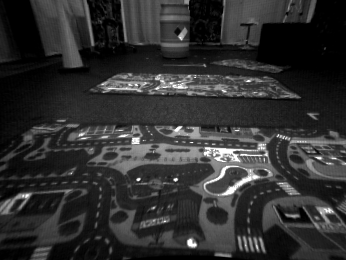
\includegraphics[width=.30\textwidth,height=1.85cm,keepaspectratio]{figures/mvsec_indoor_flying_2_alpha_10_vox_focus/gray_0340.png}&
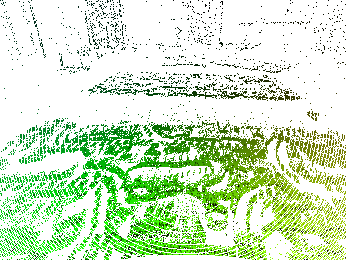
\includegraphics[width=.30\textwidth,height=1.85cm,keepaspectratio]{figures/mvsec_indoor_flying_2_alpha_10_vox_focus/flow_gt_0340.png}&
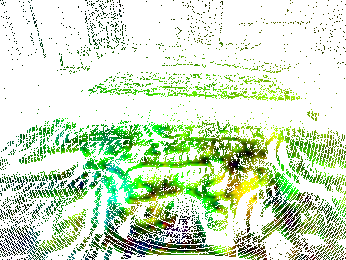
\includegraphics[width=.30\textwidth,height=1.85cm,keepaspectratio]{figures/mvsec_indoor_flying_2_alpha_10_vox_focus/flow_acc_0340.png}\\
Reference&Ground truth&Event-accumulation baseline\\[2mm]
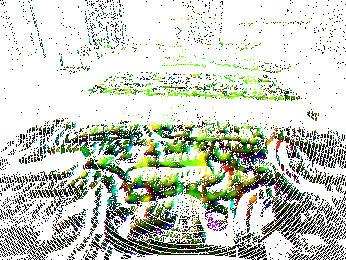
\includegraphics[width=.30\textwidth,height=1.85cm,keepaspectratio]{figures/mvsec_indoor_flying_2_alpha_10_vox_focus/flow_ts_0340.png}&
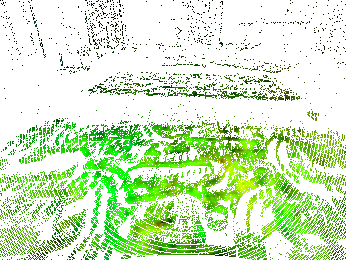
\includegraphics[width=.30\textwidth,height=1.85cm,keepaspectratio]{figures/mvsec_indoor_flying_2_alpha_10_vox_focus/flow_vox_0340.png}&
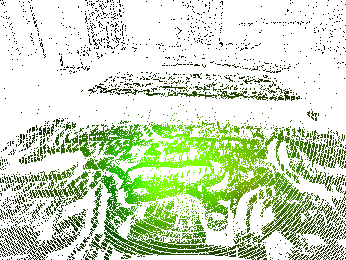
\includegraphics[width=.30\textwidth,height=1.85cm,keepaspectratio]{figures/mvsec_indoor_flying_2_alpha_10_vox_focus/flow_vox_struct_0340.png}\\
Time surface&Voxel&Structure tensor voxel
\end{tabular}
\takeaway{This is one qualitative example; Chapter 3 reports no aggregate real-data AEE.}
\src{Ch. 3, fig:vox\_comparison.}
\talknote{Question: what is the real-data AEE?}{The dissertation does not report an aggregate real-data AEE for this comparison. State that directly; no value is available in the reported results.}{The event-accumulation baseline is a separate comparison method. The theorem's coefficient representations are the time-surface, voxel, and structure-tensor constructions. These panels support a qualitative comparison only and establish no numerical ranking.}
\end{frame}

\begin{frame}{Quadratic $H^1$ regularization and TV answer different questions}
\small
The flow energy uses a quadratic gradient penalty:
% source: Ch. 3 common existence/stability theorem; abstract signed-linear quadratic energy.
\[E(\vct)=\tfrac12\int_\Omega\bigl(\vct^\top\B\vct-2b^\top\vct\bigr)
+\tfrac{\alpha^2}{2}\norm{\nabla\vct}_{L^2}^2,\qquad \vct\in H^1(\Omega;\R^2).\]
\begin{itemize}
\item Lax--Milgram gives existence, uniqueness, and coefficient stability under the stated hypotheses.
\item TV can preserve jumps, but needs a separate $BV$ existence argument and its own uniqueness and stability assumptions.
\item Normalized NE diffusion gives directional quadratic smoothing with a uniform ellipticity floor.
\end{itemize}
\takeaway{The integrated full-rank condition supports the quadratic $H^1$ proof; it does not establish a TV theorem.}
\src{Ch. 3, thm:unified\_wellposedness, function-space remark, eq:ne\_tensor.}
\talknote{Question: why use $H^1$ instead of TV?}{The quadratic model yields a bilinear form to which Lax--Milgram applies, then an energy identity gives coefficient stability. TV may retain discontinuities, but requires a separate existence framework in $BV$.}{A residual-square fidelity may be considered for a TV model, but no such theorem is established here. Replacing the gradient term with TV in an abstract signed-linear energy can make it unbounded below. Full-rank pointwise fidelity can retain strict convexity, so TV does not always lose uniqueness; the integrated condition alone no longer supplies $H^1$ coercivity.}
\end{frame}

\begin{frame}{Frozen prediction weights are not generally an MM majorizer}
For a scalar prediction $s$, let $v(s)=|s|+\varepsilon$, $\varepsilon>0$, and
% source: Ch. 4 sec:irls_scope and prop:irls_vs_nll; derivative is direct differentiation away from s=0.
\[S(s)=\frac{(y-s)^2}{2v(s)}+R(s),\qquad
Q_k(s)=\frac{(y-s)^2}{2v(s_k)}+R(s).\]
The frozen surrogate matches $S$ at $s_k$, but away from $s=0$ its derivative omits
% source: Ch. 4 sec:irls_scope; derivative of the state-dependent variance term.
\[ -\frac{v'(s)(y-s)^2}{2v(s)^2}.\]
\takeaway{Without a tangent derivative, the frozen quadratic is not generally a differentiable tangent majorizer.}
\src{Ch. 4, sec:irls\_scope, prop:irls\_vs\_nll; derivative consequence, not a stated MM theorem.}
\talknote{Question: is this IRLS a majorization-minimization method?}{In general, no. The state-dependent variance contributes the displayed derivative term, which the frozen-weight quadratic omits. Thus matching the objective value at the current iterate does not give a differentiable tangent majorizer.}{No generic descent guarantee follows. The proved existence and conditional contraction results concern a fixed map. The implementation's cost-rise acceptance rule is separate and can allow small rises, so do not claim monotone cost decrease.}
\end{frame}

\begin{frame}{A Gaussian model gives an evidence interpretation of attenuation}
For common fixed $\Lam\succ0$, $\gamma\ge0$, and independent unit Gaussian noise, the candidate conditional is
% source: supplementary derivation from Ch. 4, prop:correct_selection; P and T are defined there.
\[\mathbf y_R\mid\mathbf y_L\sim\mathcal N(\mathbf c,(2\mathbf P)^{-1}),\qquad
\mathbf c=\mathbf P^{-1}\mathbf T\mathbf y_L.\]
Coupled versus independent evidence satisfies
% source: supplementary Gaussian derivation from Ch. 4 matching-cost decomposition.
\[-\log\frac{p_\gamma(\mathbf y_L,\mathbf y_R)}{p_0(\mathbf y_L,\mathbf y_R)}
=D(\mathbf y_L-\mathbf y_R)+\text{constant}.\]
\takeaway{The conditional mean explains attenuation; the discrepancy alone is an unevaluated alternative score.}
\src{Supplementary Gaussian derivation from Ch. 4, lem:matching\_cost\_closed\_form, prop:correct\_selection.}
\talknote{Question: can attenuation be read probabilistically?}{For fixed common parameters, interpret the magnitude and coupling penalties as a Gaussian prior and observations as independent unit-noise Gaussian measurements. The conditional distribution makes the profile prediction and its uncertainty explicit.}{The prior precision is $\M_0=\left(\begin{smallmatrix}\Lam^2+\gamma I&-\gamma I\\-\gamma I&\Lam^2+\gamma I\end{smallmatrix}\right)$, and $\M=\M_0+\operatorname{diag}(\A,\A)^\top\operatorname{diag}(\A,\A)$. Integrating out the profiles gives $-\log p_\gamma(\mathbf y)=C_\gamma(\mathbf y)+\tfrac12\log\det\M-\tfrac12\log\det\M_0+\text{constant}$; these determinant terms are fixed across candidates. The operator $\mathbf P^{-1}\mathbf T$ has eigenvalues in $[0,1)$ and is self-adjoint and contractive in the $\mathbf P$ metric, but need not contract in Euclidean norm. For scalar $\Lam$, attenuation is diagonal in the temporal observation eigenmodes. The criterion from $D$ alone selects an ideal match for $\gamma>0$, full-row-rank $\A$, and distinct candidate profiles; it is an unevaluated score alternative, not a disparity MAP result or evaluated method.}
\end{frame}

\begin{frame}{The implemented estimator has several distinct layers}
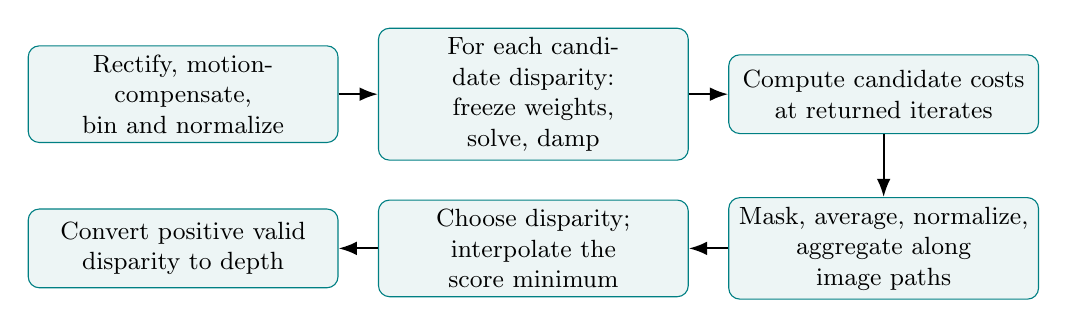
\begin{tikzpicture}[>=Latex,node distance=4mm,every node/.style={font=\small},box/.style={draw=teal,fill=soft,rounded corners,align=center,text width=3.7cm,minimum height=1cm}]
\node[box] (a) {Rectify, motion-compensate,\\bin and normalize};
\node[box,right=5mm of a] (b) {For each candidate disparity:\\freeze weights, solve, damp};
\node[box,right=5mm of b] (c) {Compute candidate costs\\at returned iterates};
\node[box,below=8mm of c] (d) {Mask, average, normalize,\\aggregate along image paths};
\node[box,left=5mm of d] (e) {Choose disparity;\\interpolate the score minimum};
\node[box,left=5mm of e] (f) {Convert positive valid\\disparity to depth};
\draw[->,thick] (a)--(b);\draw[->,thick] (b)--(c);\draw[->,thick] (c)--(d);\draw[->,thick] (d)--(e);\draw[->,thick] (e)--(f);
\end{tikzpicture}
\vspace{4mm}
Theorems describe specific layers; empirical evaluation describes the complete estimator.
\takeaway{The exact minimum of a computed score list is not a certificate of the true disparity or of a global image-level energy minimum.}
\src{Ch. 4, sec:solution; Appendix, app:protocol\_ch4.}
\talknote{Implementation scope; 60 seconds.}{Expand IRLS as iteratively reweighted least squares and SGM as semi-global matching: SGM penalizes disparity changes along multiple paths to encourage spatial coherence. A finite search exactly returns a minimum of the final score list, subject to tie breaking. That narrow exactness should not be confused with correctness of the physical correspondence or exact optimization of a global two-dimensional labeling energy.}{Clipping affects solve weights; final scores recompute unclipped weights. Finite penalty sentinels are averaged before selection, so the guidance window is soft. The benchmark includes the finest-level interpolation of the aggregated score but excludes the separate hole-filling/refinement operator. A detailed audit of these layers is in the backup.}
\end{frame}

\begin{frame}{What does the dissertation contribute mathematically?}
\begin{itemize}
\item A transparent temporal inversion with an explicit observation null space and quantitative fixed-weight guarantees.
\item One well-posedness and stability theorem for several event-derived quadratic flow energies, with representation-specific hypotheses.
\item A distinction between a coercive spline regularizer and a nonconvex contrast objective, plus full-objective existence.
\item Stereo block structure, profiled-cost bias, ideal selection and robustness criteria, and a scoped adaptive-weight analysis.
\end{itemize}
\takeaway{Classical proof tools connect the models; the event-specific formulation, hypotheses, consequences, and limitations are the research content.}
\src{Chs. 1 and 5; labeled results throughout Chs. 2--4.}
\talknote{Question: what is new if the proof tools are classical?}{Do not claim to invent Tikhonov regularization, Horn--Schunck, Lax--Milgram, or Brouwer. Explain the work as constructing and comparing precise event-based inverse models, identifying what assumptions make them well posed, and deriving consequences that are otherwise easy to overclaim. The common flow theorem gives a reusable treatment instead of separate incomplete proofs.}{The stereo cost decomposition and attenuation example explain why inner solvability does not guarantee correct correspondence. The separation and margin conditions supply a conditional answer. The fixed/adaptive split prevents a quadratic guarantee from being incorrectly transferred to a changing-weight procedure. These are concrete mathematical insights that inform model design and evaluation.}
\end{frame}

\begin{frame}{Literature anchors and where to find the claims}
\small
\begin{itemize}
\item \textbf{Sensor and field overview:} Gallego et al., \emph{Event-based Vision: A Survey}; dissertation bibliography key \texttt{gallego2022event}.
\item \textbf{Variational flow:} Horn and Schunck, \emph{Determining Optical Flow}; \texttt{horn1981determining}.
\item \textbf{Timestamp geometry:} Benosman et al., \emph{Event-Based Visual Flow}; \texttt{benosman2014event}.
\item \textbf{Contrast maximization:} Gallego, Rebecq, and Scaramuzza, \emph{A Unifying Contrast Maximization Framework}; \texttt{gallego2018unifying}.
\item \textbf{Evaluation data:} Zhu et al., \emph{The Multivehicle Stereo Event Camera Dataset}; \texttt{MVSEC2018}.
\end{itemize}
\vspace{2mm}
Every slide's footer identifies its dissertation source. The companion source map records theorem labels, current theorem numbers, figures, numerical tables, and scope.
\src{GMU-Diss\_template.tex; gmuETD.bib; Ch. 3 related work; Appendix evaluation protocol.}
\talknote{Attribution.}{These are literature anchors for the sensor model, classical flow framework, time-surface approach, event warping, and dataset. The talk's empirical numbers and theorem statements are drawn from the local dissertation, not assembled from an external search or new experiments.}{Dissertation label names are more durable than current page or theorem numbers, which can shift when the manuscript is edited. The source map provides both where available.}
\end{frame}

\begin{frame}{Stable estimates can still have regularization bias}
For fixed scalar $\lambda>0$, $\mathbf y=\A\mathbf f^\dagger+\boldsymbol\eta$, and $\K=\A^\top\A+\lambda^2\mathbf I$,
% source: Ch. 2 thm:uniqueness, prop:stability; bias-noise split follows by direct substitution.
\[\mathbf f_\lambda-\mathbf f^\dagger
=-\lambda^2\K^{-1}\mathbf f^\dagger+\K^{-1}\A^\top\boldsymbol\eta.\]
The two terms are regularization bias and propagated observation noise.
\takeaway{A stable estimate need not equal the physical signal.}
\src{Ch. 2, thm:uniqueness, prop:stability; direct bias-noise identity.}
\talknote{Question: does stability imply truth?}{No. The estimator's error splits into a shrinkage bias and propagated noise. The stability bound controls sensitivity to the observations, while the bias depends on the signal and the penalty.}{A zero-mean reference fixes the unobservable constant ambiguity. On a fixed grid, noiseless data from a mean-zero reference signal are recovered as $\lambda\to0$. Persistent noise can prevent recovery as $\lambda\to0$; uniform refinement requires controlling noise, regularization, and grid scaling. Model error may enter the residual separately from sensor noise.}
\end{frame}

\begin{frame}{The physical event stream loses more than one baseline}
The binned increment matrix has $\ker\A=\operatorname{span}\{\mathbf1\}$, but the ideal sensor can lose time-varying signals too.
% source: Ch. 2 eq:polarity; zero-event pair below is a direct ideal-threshold illustration.
\[L_1(t)=L_0,\qquad L_2(t)=L_0+a\sin(2\pi t/T),\qquad
0<a<c_{\rm th},\quad t\in[0,T].\]
Both start at $L_0$, emit no events, and have positive intensities $I_j(t)=e^{L_j(t)}$.
\takeaway{The chain nullspace describes the discrete increment surrogate, not every ambiguity of the physical sensor.}
\src{Ch. 2, eq:polarity, lem:nullspace; direct ideal-sensor example.}
\talknote{Question: is the constant nullspace the whole sensor ambiguity?}{No. The chain matrix has exactly the constant nullspace, but the sensor only fires after a contrast threshold crossing. The two displayed positive intensity signals share the same initial reference and remain inside that threshold, so both produce the same empty event stream.}{This example shows that a physical stream can omit changes that never cross threshold. It does not say arbitrary perturbations preserve a nonempty event schedule. A small perturbation supported strictly away from existing crossings can preserve that schedule when there is a positive threshold margin.}
\end{frame}

\begin{frame}{Integrated directional information is necessary for uniqueness}
Let $\Omega$ be connected, bounded, and Lipschitz; $\alpha>0$; $\B\in L^\infty$ symmetric PSD; and $b\in L^2$. Minimize over unrestricted $H^1(\Omega;\R^2)$ fields. Set $M_B=\int_\Omega\B$.
% source: Ch. 3 thm:unified_wellposedness; the converse follows directly for its quadratic energy.
If $M_B$ is singular, choose $c\ne0$ with $M_Bc=0$. Then $\B c=0$ a.e. and
\[E(\vct+tc)=E(\vct)-t\,c^\top\!\int_\Omega b.\]
If the coefficient is nonzero, $E$ is unbounded below; if zero, it is flat in direction $c$.
\takeaway{The integrated matrix condition is necessary for a unique minimizer in this unrestricted quadratic model.}
\src{Ch. 3, thm:unified\_wellposedness; direct converse for its quadratic energy.}
% source: Ch. 3 thm:unified_wellposedness; PSD plus zero integral of c^T B c forces Bc=0 a.e.
\talknote{Question: why require $\int\B\succ0$?}{A singular integrated matrix leaves a nonzero constant flow direction unseen by both the data quadratic and the gradient penalty. Along that direction, the remaining linear term either drives the energy without a lower bound or vanishes.}{Because $\B$ is PSD, $c^\top\B(x)c\ge0$ a.e.; its integral is $c^\top M_Bc=0$, so $\B^{1/2}c=0$ and hence $\B c=0$ a.e. In the zero-slope case, any existing minimizer would have a flat family, so uniqueness fails; this alone does not prove a minimizer exists. Residual-square data can make the linear coefficient compatible with the null direction. Boundary constraints or a ridge term change the argument.}
\end{frame}

\begin{frame}{Coefficient stability is one stage of event-to-flow stability}
\centering
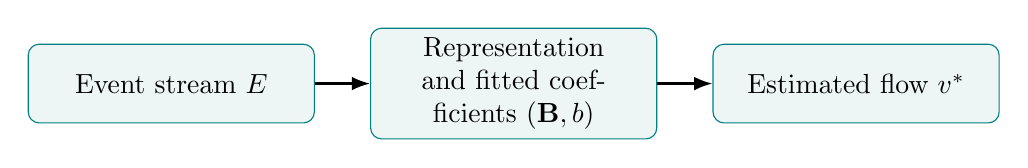
\begin{tikzpicture}[>=Latex,node distance=7mm,every node/.style={draw=teal,fill=soft,rounded corners,align=center,text width=3.4cm,minimum height=1cm}]
\node (a) {Event stream $E$};
\node[right=of a] (b) {Representation and fitted coefficients $(\B,b)$};
\node[right=of b] (c) {Estimated flow $v^*$};
\draw[->,thick] (a)--(b);\draw[->,thick] (b)--(c);
\end{tikzpicture}
\par
% source: Ch. 3 thm:unified_wellposedness and prop:ts_regression_bound; composition is a scope observation.
\vspace{4mm}
The theorem controls coefficient-to-flow sensitivity. A Lipschitz representation map could compose with that bound.
\takeaway{An end-to-end guarantee also needs a metric and stability result for event preprocessing.}
\src{Ch. 3, thm:unified\_wellposedness, prop:ts\_regression\_bound; supplementary scope explanation.}
% source: supplementary metric illustration for one positive unit atom; total variation norm uses measure variation.
\talknote{Question: how stable is the full event-to-flow pipeline?}{The variational theorem begins after events have become coefficient fields. If preprocessing were Lipschitz in a chosen event metric, its bound could compose with the coefficient-to-flow estimate.}{The metric matters: moving one positive unit atom by nonzero $\delta t$ gives the total variation norm $\lVert\delta_{t+\delta t}-\delta_t\rVert_{\rm TV}=2$, while the single-atom mass-one Wasserstein distance is $|\delta t|$. Hard bins or changing candidate neighborhoods may jump; fixed-bandwidth smoothing can behave better under a suitable metric. No global pipeline theorem is established here.}
\end{frame}

\begin{frame}{Refinement requires a choice of continuum scaling}
\small
Illustrative smooth, uniform-time model only: spacing $h$, increments $y_i=h g_i$, and target energy
% source: Ch. 2 eq:tempdiffA, eq:in; continuum quadrature scaling is a supplementary derivation.
\[\frac12\int|f'-g|^2dt+\frac{\beta_{\rm time}^2}{2}\int|f|^2dt
\quad\leadsto\quad
\frac1{2h}\norm{\A f-y}^2+\frac{\beta_{\rm time}^2h}{2}\norm{f}^2.\]
Multiplying the discrete objective by $h$ gives the Chapter 2 form with
% source: direct coefficient matching to Ch. 2 eq:in.
\[\lambda_h=\beta_{\rm time}h.\]
\takeaway{The penalty's grid scaling depends on the continuum objective being approximated.}
\src{Ch. 2, eq:tempdiffA, eq:in; supplementary smooth-model scaling illustration.}
\talknote{Question: should $\lambda$ change as the grid is refined?}{There is no answer without naming a target continuum functional. In this smooth uniform-time illustration, difference residuals scale like $h$, while the Riemann sum contributes $1/h$. Matching the magnitude penalty yields $\lambda_h=\beta_{\rm time}h$.}{Finite-endpoint quadrature may need endpoint weights, and this calculation is not a convergence theorem. A physical event model would also require a scaling choice for noise and kernel bandwidth. It does not assert that the dissertation's finite-grid experiments must use this law.}
\end{frame}

\begin{frame}{Strong smoothness selects one constant flow}
For fixed $\Omega,\B,b$ satisfying the unified theorem, with unrestricted $H^1$ fields and the same $\alpha^2$ gradient coefficient,
% source: Ch. 3 thm:unified_wellposedness; the alpha-to-infinity limit is a direct corollary derivation.
\[\alpha\to\infty\quad\Longrightarrow\quad
v_\alpha\to c\text{ in }H^1,\qquad
c=\left(\int_\Omega\B\right)^{-1}\int_\Omega b.\]
\takeaway{Very strong spatial regularization removes variation and leaves the data-balanced constant field.}
\src{Ch. 3, thm:unified\_wellposedness; direct strong-regularization limit.}
% source: Ch. 3 thm:unified_wellposedness; direct estimate from its weak equation and Poincare inequality.
\talknote{Question: what happens as $\alpha$ grows?}{The gradient penalty forces the minimizer toward a constant field. The data term then selects the constant that balances the integrated directional information against the integrated forcing.}{For a proof, write $w_\alpha=v_\alpha-c$ and test the weak equation with it. With $h_b=b-\B c$ and $\int h_b=0$, the identity is $\int w^\top\B w+\alpha^2\norm{\nabla w}_2^2=\int h_b\cdot(w-\bar w)$. Poincare gives $\norm{\nabla w}=O(\alpha^{-2})$. Testing constants yields $\int\B w=0$; positive definiteness of $\int\B$ and Poincare then give $\bar w\to0$. This is a direct corollary, not a separately stated theorem. No blanket $\alpha\to0$ claim follows.}
\end{frame}

\begin{frame}{Transporting a scalar differs from conserving a density}
Scalar transport and source-free density conservation are
% source: Ch. 3 subsec:vox_projection and sec:vox_cont_exclusion; product rule is direct.
\[V_t+v\cdot\nabla V=0,\qquad
V_t+\nabla\cdot(Vv)=0,\qquad
\nabla\cdot(Vv)=v\cdot\nabla V+V\,\nabla\cdot v.\]
They coincide when $V\nabla\cdot v=0$, in particular for divergence-free flow.
\takeaway{The continuity equation adds a density-compression term to scalar transport.}
\src{Ch. 3, subsec:vox\_projection, sec:vox\_cont\_exclusion; direct product-rule comparison.}
% source: Ch. 3 sec:vox_cont_exclusion; one-dimensional v=x, V=1 is a direct illustration.
\talknote{Question: should events be modeled as a conserved fluid?}{That is an additional physical assumption. Scalar transport follows a pattern value along a trajectory; density conservation also accounts for compression or expansion through the divergence of flow.}{For a simple illustration, in one dimension let $v(x)=x$ and $V(x,t)=1$. It solves scalar transport, but source-free conservation has residual $\partial_x(Vv)=1$. A source term $V_t+\nabla\cdot(Vv)=s$ may be appropriate if events are created or lost, but this dissertation establishes no physical event conservation law.}
\end{frame}

\begin{frame}{Correlation changes uncertainty without removing coercivity}
For a centered symmetric regression design $Z$ with $Q=Z^\top Z\succ0$, timestamp-error covariance $\Sigma$ gives
% source: Ch. 3 prop:ts_regression_bound; covariance identity is the direct OLS extension to correlated errors.
\[\operatorname{Cov}(\hat g)=Q^{-1}Z^\top\Sigma ZQ^{-1}.\]
This reduces to $\sigma^2Q^{-1}$ when $\Sigma=\sigma^2 I$.
\par\medskip
% source: Ch. 2 eq:in and thm:uniqueness; positive definite fidelity matrix preserves SPD.
With any $\Gamma\succ0$, the temporal system matrix is $\A^\top\Gamma^{-1}\A+\Lam^2\succ0$ when $\Lam\succ0$.
\takeaway{The deterministic quadratic solve stays coercive, while statistical uncertainty depends on the error covariance.}
\src{Ch. 3, prop:ts\_regression\_bound; Ch. 2, eq:in, thm:uniqueness; direct correlated-error extension.}
% source: direct OLS linear-map covariance; Ch. 2 thm:uniqueness for weighted SPD normal matrix.
\talknote{Question: what if timestamp errors are correlated?}{Independence is not needed for the covariance formula of a linear OLS estimator; the full covariance matrix replaces the white-noise simplification. If each error has the same mean, the centered symmetric design cancels that mean in the slope.}{Smoothing errors with $H_\epsilon$ produces $H_\epsilon\Sigma H_\epsilon^\top$, which may be singular, so do not invert it without checking. A positive definite fidelity precision $\Gamma^{-1}$ keeps the regularized normal matrix positive definite, but changes coefficients and constants. A Gaussian likelihood interpretation needs a separate distributional assumption; the deterministic theorem does not validate a noise model.}
\end{frame}

% Preserved from core as discussion-only material when the main talk foregrounded
% adaptive-weight selection and the Chapter 2 bilevel comparison.
\begin{frame}{What the penalty does to temporal information}
For scalar $\Lam=\lambda\mathbf I$ and noiseless data $\mathbf y=\A\mathbf f_{\rm true}$:
% source: Ch. 4 lem:A_spectrum, thm:frequency_response; same first-difference matrix as Ch. 2.
\[g_k=4\sin^2\!\frac{\pi k}{2n},\qquad H_k=\frac{g_k}{g_k+\lambda^2},\qquad H_0=0.\]
\begin{columns}[c]
\column{.55\textwidth}
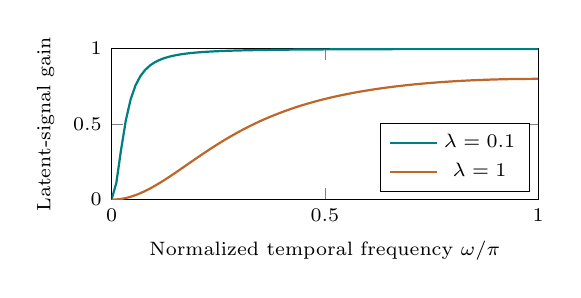
\begin{tikzpicture}
\begin{axis}[width=7cm,height=3.5cm,xmin=0,xmax=1,ymin=0,ymax=1,xtick={0,.5,1},ytick={0,.5,1},xlabel={Normalized temporal frequency $\omega/\pi$},ylabel={Latent-signal gain},label style={font=\scriptsize},tick label style={font=\scriptsize},legend style={font=\scriptsize,at={(.98,.05)},anchor=south east}]
% source: analytic continuous extension H(omega) in Ch. 4 eq:transfer_function; chosen illustrative lambda values.
\addplot[teal,thick,domain=0:1,samples=90]{4*sin(90*x)^2/(4*sin(90*x)^2+.01)};\addlegendentry{$\lambda=0.1$}
\addplot[amber,thick,domain=0:1,samples=90]{4*sin(90*x)^2/(4*sin(90*x)^2+1)};\addlegendentry{$\lambda=1$}
\end{axis}
\end{tikzpicture}
\column{.42\textwidth}
The baseline is removed.\par\medskip
Low temporal modes are attenuated most.\par\medskip
A unique estimate does not restore the missing physical baseline.
\end{columns}
\src{Ch. 4, lem:A\_spectrum, thm:frequency\_response. Curves: continuous extension.}
\talknote{Spectral interpretation; 75 seconds.}{The first-difference Gramian is the Neumann-chain Laplacian. Its constant eigenvector has eigenvalue zero. Expanding a noiseless latent signal in the eigenbasis turns reconstruction into multiplication by g/(g+lambda\textasciicircum{}2). These are latent-signal gains; the gain from noise in the difference observations is a different expression in the backup.}{The spectral decomposition is proved in Chapter 4 and reused here for stereo. The plotted smooth curves interpolate the finite-chain modal gains. Only omega\_k=pi k/n are exact finite-grid modes. This magnitude penalty attenuates low temporal frequencies most, whereas the temporal kernels may average rapid changes.}
\end{frame}

\begin{frame}{Temporal evidence: structure without an absolute baseline}
\begin{columns}[c]
\column{.55\textwidth}
\panel{.48}{figures/mvsec_outdoor_day1/bump_sweep/ground_truth/ground_truth_frame076.png}{Reference}
\hfill\panel{.48}{figures/mvsec_outdoor_day1/bump_sweep/sample_reconstructions/mvsec_outdoor_day1_subset_bspline_order1p000_width0p010_param1_frame076.png}{Spline reconstruction}
\column{.42\textwidth}
\small MVSEC indoor kernel comparison\par\medskip
\begin{tabular}{lrr}\toprule Kernel & PSNR & CN\\\midrule
% source: Ch. 2 tab:bump_avg_indoor, PSNR and CN columns; displayed rounded values copied.
B-spline & 8.86 & 22.16\\
% source: Ch. 2 tab:bump_avg_indoor, Delta row.
Delta & 7.70 & 1375.75\\
% source: Ch. 2 tab:bump_avg_indoor, Gaussian row.
Gaussian & 8.84 & 20.22\\\bottomrule
\end{tabular}
\end{columns}
\takeaway{Kernel and adaptive-weight choices affect both the reconstruction and the solved system.}
\src{Ch. 2, tab:bump\_avg\_indoor and outdoor bump-sweep gallery. CN: reported condition number.}
% source: Ch. 2 tab:bump_avg_indoor; CN values and source-limited PSNR interpretation.
\talknote{Temporal results; 60 seconds.}{The pictures are an outdoor example; the compact table is an indoor aggregate. Say that distinction explicitly. PSNR is a reference-image similarity measure and CN the reported system condition number. The dissertation reports these values descriptively; the available historical sources do not recover the PSNR normalization or alignment protocol.}{No general guarantee says a spline always improves conditioning or reconstruction. The outdoor table has a different ordering, included in the backup. The scores are not proof of absolute-intensity recovery. The shown CN range is 20.22--1375.75: Gaussian 20.22, B-spline 22.16, Delta 1375.75. Display normalization and false color are visualization choices, not measured absolute brightness.}
\end{frame}

\end{document}
